\documentclass[11pt]{article}
\usepackage[english]{babel}
%\usepackage{natbib}
\usepackage{url}
\usepackage{float}

\usepackage{amssymb}
\usepackage{amsfonts}
\usepackage{booktabs}
\usepackage{hyperref}
\usepackage{rotating}
\usepackage{appendix}
\usepackage[utf8x]{inputenc}
\usepackage{amsmath}
\usepackage{graphicx}
\usepackage{color}
\usepackage{transparent}
\usepackage{parskip}
\usepackage{fancyhdr}
\usepackage{background}

% use an images folder
\graphicspath{{images/}}

\usepackage[a4paper, total={165mm, 216mm}]{geometry}
\renewcommand{\familydefault}{\sfdefault}

% set running headings on each page
% https://www.overleaf.com/learn/latex/Headers_and_footers
\pagestyle{fancy}
\rhead{\theauthor}
\lhead{\subtitle}
\cfoot{\thepage}
\backgroundsetup{contents={}}
\begin{document}

  % --- edit ---
\author{G.V. Vetsler} % author
\title{Comparing classical and neural collaborative filtering models on implicit feedback data} % title
\newcommand\subtitle{Comparing collaborative filtering models} % subtitle
\newcommand\supervisor{Dr. Marijn, Jansen
} % supervisor
\newcommand\secondexaminer{Dr. Tamas, Vinko
} % second examiner
\newcommand\studentnumber{9783954} % student number
\date{\today} % date

% adjust to a number between 1-2 only if title is long does not fit on page
\newcommand\titlespace{2}

% --- do not edit ---
\makeatletter
\let\thetitle\@title
\let\theauthor\@author
\let\thedate\@date
\let\thespace\@titlespace
\makeatother

\begin{titlepage}
\backgroundsetup{
  scale=1,
  angle=0,
  opacity=0.5,
  contents={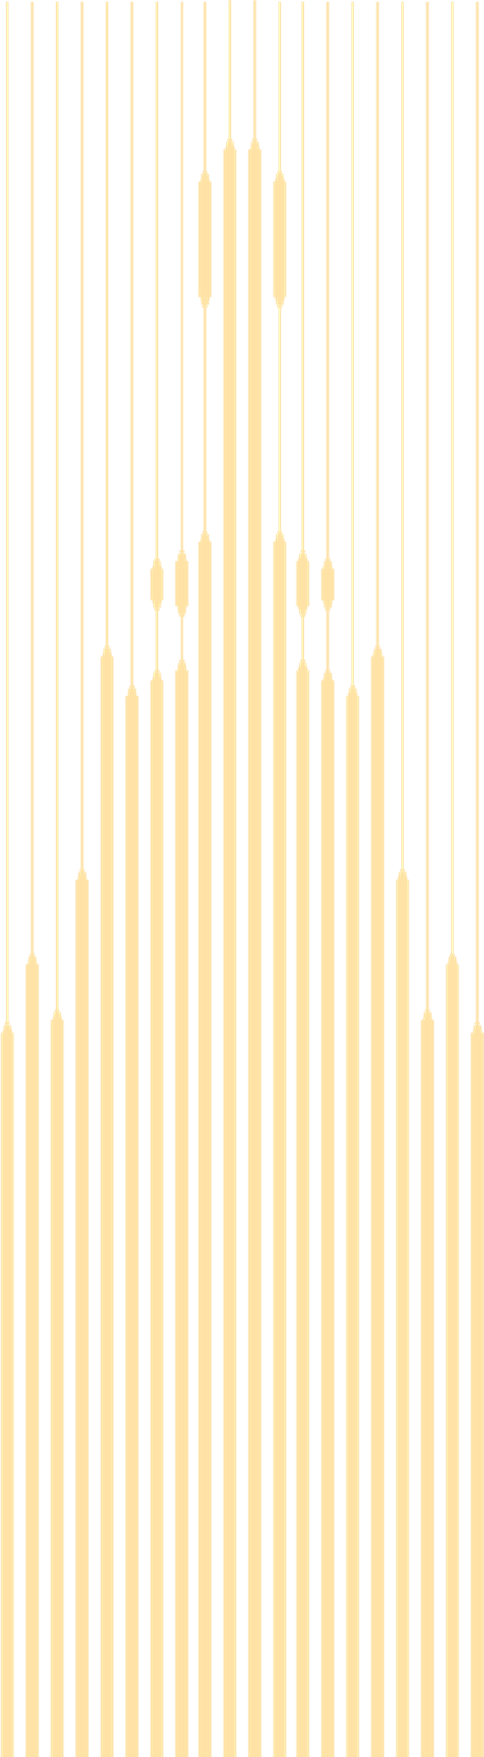
\includegraphics[height=1.05\paperheight]{images/bg.png}},
  position={14,-12.4}, % flush right, full height
}

\noindent
\begin{picture}(0,0)
    \put(-20,-40){\transparent{0.5}
\includegraphics[height=3.5cm]{UCRlogo.png}}
\end{picture}
\begin{flushleft}
\vspace*{1.5 cm}
{\LARGE University College Roosevelt}\\[0.4 cm]
{\large Lange Noordstraat 1, Middelburg, The Netherlands}\\[0.4 cm]
{\large Bachelor of Liberal Arts \& Sciences}\\[\titlespace cm]
{\Huge Senior Project}\\[0.2 cm]
\rule{\linewidth}{0.2 mm} \\[0.4 cm]
{\Huge \thetitle}\\[0.6 cm]
{\LARGE \subtitle} \\
\rule{\linewidth}{0.2 mm} \\[\titlespace cm]

\begin{minipage}[t]{0.45\textwidth}
\large
\textbf{Author:}\\[0.1cm]
\theauthor\\[0.1cm]
\studentnumber\;(Student Number)\\[0.5cm]
\textbf{Supervisor:}\\[0.1cm]
\supervisor\\[0.5cm]
\textbf{Second examiner:}\\[0.1cm]
\secondexaminer\\[\titlespace cm]
{\large \thedate}
\end{minipage}

\vfill
\end{flushleft}

\end{titlepage}
  



\pagebreak
\begin{abstract}



Collaborative Filtering (CF) remains a fundamental component of modern recommender systems, recently evolving from classical Matrix Factorization (MF) techniques to deep learning-based architectures such as Neural Matrix Factorization (NeuMF)~\cite{he2017neural} and Convolutional Neural Collaborative Filtering (ConvNCF) ~\cite{he2018convncf}, both of which claim substantial improvements over classical matrix factorization and neighborhood baselines on implicit-feedback benchmarks. At the same time, recent critical studies argue that many neural recommenders offer limited accuracy gains that do not justify their added complexity, especially when compared to strong baselines and careful tuning of baseline models ~\cite{rendle2020neural,anelli2021reenvisioning}. This thesis revisits these claims by conducting a controlled empirical comparison, under computational and time limits, of NeuMF, a shallow ConvNCF variant, and several baseline models on two widely used datasets, MovieLens-1M and Yelp.


The experimental setup includes Item-based K-Nearest Neighbors (ItemKNN), Matrix Factorization with Bayesian Personalized Ranking (MF-BPR), and several neural recommendation models. The neural models cover Generalized Matrix Factorization (GMF), an MLP-based recommender, NeuMF (both with and without pretraining), and a shallow ConvNCF model that uses outer-product interaction maps.

The results show that shallow embedding-based models such as GMF consistently match or outperform more complex neural architectures on MovieLens, while on Yelp a simple ItemKNN baseline yields the best accuracy. NeuMF-pre achieves competitive but not dominant performance, and ConvNCF performs poorly on MovieLens and only moderately well on Yelp despite its higher complexity. These findings support recent critiques that very deep neural architectures are not necessarily the best choice collaborative filtering problems. In this setting, well-regularised MF-style and neighbourhood methods remain strong and often preferable baselines.
\end{abstract}
\tableofcontents



%Talk about the importance of reccomender models on implicit data, with real world examples

%talk about the implementation of NeuMF model
%talk about what questions are stated (the ones from the combined results), and a bit of litiriture that talk about same things


%Talk more about which models were implemented



\section{Introduction}

Modern online platforms, like Netflix, Spotify, TikTok operate at a scale where users are exposed to thousands of potentially relevant items every day. The success of these businesses critically depends on the quality of recommendations—be they movies, songs, or short-form videos—delivered to their users. Thus, Recommender systems (RS) are a critical component of such platforms, that have to filter all of the incoming data and produce an accurate prediction of personalized ranked list of items for the user.

Most of the data is stored in the implicit user-item interaction data (can be clicks, views). Learning from implicit data is, however, more challenging: the absence of interaction does not necessarily indicate dislike, it often indicates that the user just has not interacted with it. Designing effective collaborative filtering models for this setting is therefore both practically important and methodologically complex.

To better understand the advancements of the RSs an extensive and broad literature review was conducted on different advancements in RSs before and after introduction of NeuMF model. 

The traditional approach to collaborative filtering has been latent factor models such as matrix factorization (MF), which represent users and items as low-dimensional embeddings and estimate relevance via an inner product between these vectors. While MF has proven highly effective, the inner product imposes a strong inductive bias: it assumes that embedding dimensions contribute independently and linearly to the final score. This simplicity can be too restrictive when the true user–item interaction patterns are more complex. This limitation has motivated to come up with flexible neural architectures, that better capture the non-linear relationships in the data.

Neural Collaborative Filtering (NCF) addresses this limitation by learning the interaction function between user and item embeddings with deep neural networks. The NeuMF model combines a generalized MF component (GMF) with a multi-layer perceptron (MLP): an element-wise product branch preserves the inductive bias of MF, while a parallel MLP branch operates on concatenated embeddings to capture non-linear interactions. The two branches are fused at the prediction layer and trained end-to-end on implicit feedback with a classification-aware loss, which potentially can lead to consistent improvements over strong MF baselines.

Another idea in CFs, is the Outer Product-based NCF (ONCF) and its ConvNCF instantiation have been proposed as an alternative neural architecture. Instead of concatenation or element-wise product, ConvNCF applies an outer product to form a two-dimensional interaction map \ref{fig:heat_map_movie} between embedding dimensions and then uses a convolutional neural network to try to capture spatial patterns of the interaction map.

On the other hand, there is some critique of the deep learning methods applied to CF, especially on NeuMF and ConvNCF models. This thesis aims to answer three main questions: (i) Are MLP-based models a good fit for CF data; (ii) Is ConvNCF a good fit and the outer product actually has spatial features that can be captured by CNNs; (iii) To what extent deep learning is helpful in the CF models.

This study evaluates classical models (Item-KNN, MF-BPR) against neural architectures (GMF, MLP, NeuMF, ConvNCF) by implementing them strictly as defined in the original literature \cite{he2017neural, he2018convncf}. By utilizing both the MovieLens-1M and Yelp datasets, this research extends the empirical findings of the original papers, by testing NeuMF’s performance on Yelp and ConvNCF’s performance on MovieLens—to provide a more general comparative analysis of models generalization.



\section{Literature review}
\subsection{Pre-NeuMF Recommendation Paradigms}
\label{sec:pre-neumf}
Collaborative Filtering (CF) remains the corner stone of modern recommender systems, operating on the fundamental assumption that users who interacted in a similar way in the past will do the same in the future. Prior to the milestone model -  Neural Matrix Factorization (NeuMF)~\cite{he2017neural}, the evolution of CF can be broadly categorized into three distinct eras: memory-based heuristics, latent factor models, and early neural explorations. Each generation of models try to address the type of the the relationship between user and items.  

\subsubsection{Memory-based Neighbourhood Approaches}

The earliest implementations of CF relied on memory-based strategies, which predict preferences using the user-item interaction matrix. These methods are generally divided into user-based~\cite{resnick1994grouplens,breese1998empirical} and item-based approaches~\cite{sarwar2001item,shardanand1995social}. In the user-based formulation, a target user's missing rating is estimated via a weighted aggregation of ratings from peers with high Pearson correlation or cosine similarity. Conversely, item-based CF—which gained prominence in industrial settings like Amazon—reverses this logic by computing similarities between item vectors. This proved advantageous for scalability, as item-item relationships are typically more static than user dynamics and can be pre-computed offline~\cite{sarwar2001item}.

While neighbourhood methods offer high interpretability and straightforward implementation, they are fundamentally limited by data sparsity. When the intersection of rated items between users is small, similarity measures become unreliable and recommendation quality degrades. This challenge is closely related to, and  severe in cold-start scenarios, where new users or items lack historical interactions and cannot be effectively recommended without additional data~\cite{schein2002methods}.
Furthermore, these methods rely on fixed, linear similarity measures that struggle to capture complex global patterns in user-item interactions, motivating the shift toward model-based techniques. Moreover, a significant challenge is the inherent lack of scalability, as neighbor-based models become computationally prohibitive for large datasets, since they require calculating simularities between each pair of users or items do be able to make a prediction.

\subsubsection{Latent Factor Models and Matrix Factorization}

The field underwent a paradigm shift with the adoption of Latent Factor Models, most notably Matrix Factorization (MF). Rather than relying on direct neighbour heuristics, MF characterizes users and items by mapping them into a shared, lower-dimensional latent space~\cite{koren2009matrix}. The affinity between user $u$ and item $i$ is modeled as the inner product of their latent vectors, $\hat{y}_{ui} = \mathbf{p}_u^T \mathbf{q}_i$,  transforming recommendation into a dimensionality reduction problem.

Foundational works like Probabilistic Matrix Factorization (PMF)~\cite{mnih2007probabilistic} placed this approach within a Bayesian framework to handle Gaussian noise and regularization. Extensions such as SVD++~\cite{koren2008factorization} further refined the model by incorporating implicit feedback and bias terms, significantly improving accuracy during the Netflix Prize competition. Moreover, research expanded beyond explicit rating prediction to ranking tasks; Bayesian Personalized Ranking (BPR)~\cite{rendle2012bpr} introduced a pairwise loss function optimized for implicit feedback, which remains a standard baseline for top-$N$ recommendation.

Despite its dominance, MF is inherently constrained by its interaction function. The reliance on a simple dot product assumes that latent dimensions are independent and combine linearly to form a preference. This linearity prevents the model from capturing complex, non-linear feature interactions that may exist in real-world peoples' decision processes~\cite{he2017neural}. 

\subsubsection{Early Neural Network-based CF}

As deep learning matured in computer vision and NLP, researchers began adapting neural architectures for collaborative filtering to overcome the linearity of MF. Initial efforts focused on generative models; for instance, Salakhutdinov et al.~\cite{salakhutdinov2007restricted} employed Restricted Boltzmann Machines (RBMs) to model the distribution of user ratings, demonstrating performance comparable to well-tuned SVD models.

Subsequent work leveraged autoencoders to learn non-linear representations. AutoRec~\cite{sedhain2015autorec} demonstrated that a simple autoencoder taking a user (or item) rating vector as input could reconstruct missing values with high accuracy, outperforming traditional MF. Similarly, CF-NADE~\cite{zheng2016neural} utilized a neural autoregressive architecture to model the joint probability of ratings. Other approaches, such as Neural Network Matrix Factorization (NNMF)~\cite{dziugaite2015neural}, attempted to replace the dot product with a multi-layer perceptron (MLP).

However, these early neural methods were often plagued by training difficulties and a lack of focus on ranking optimization. They typically treated the neural network as a black-box function approximator for ratings rather than designing an architecture specifically tailored to model the interaction function between user and item embeddings. Thus, there was a gap, that had to be filled with a deep learning model, tailored for specific recommender tasks.

\subsection{Post-NeuMF Developments}
\label{sec:post-neumf}
The introduction of Neural Matrix Factorization (NeuMF)~\cite{he2017neural} marked a pivotal shift in collaborative filtering (CF), demonstrating that non-linear architectures could surpass the dot-product idea of traditional Matrix Factorization related models (MF). Post-2017 research went for four different ideas: enhanced interaction modeling, graph-based learning, sequential models, and knowledge-aware combined systems.

\subsubsection{Advanced Interaction Modeling}

While NeuMF generalizes the interaction function, it does not inherently capture the explicit feature correlations found in Factorization Machines (FMs). DeepFM~\cite{guo2017deepfm} addresses this by creating a unified architecture that trains a 'wide' FM component (for low-order feature interactions) alongside a ``deep'' DNN component (for high-order interactions) without requiring manual feature engineering. The core idea is that users and items interact through both simple pairwise matches and complex non-linear patterns. 

Taking a different approach, ConvNCF (Outer Product-based NCF)~\cite{du2018convncf} argues that simply concatenating embeddings into an MLP, as in NeuMF, fails to capture explicit pairwise correlations. Instead, it computes an outer product between user and item embeddings to form a two-dimensional interaction map, which is then processed by a Convolutional Neural Network (CNN). While this explicitly models embedding-dimension correlations, the interaction map scales quadratically with embedding size, making the model computationally slow for high-dimensional representations.

Simultaneously, probabilistic methods such as Variational Autoencoders for CF (Mult-VAE)~\cite{liang2018variational} move away from point-wise estimation entirely. Mult-VAE models user history as a sample from a latent multinomial distribution, using Bayesian inference to handle the uncertainty in implicit feedback. By introducing a tunable regularization parameter (KL-annealing), it prevents overfitting on sparse data. While Mult-VAE often outperforms deterministic autoencoders, it introduces significant training complexity due to the sampling steps required for stochastic variational inference.

\subsubsection{The Graph Learning Paradigm}

Perhaps the most significant post-NeuMF evolution is the recognition that user--item data is inherently a bipartite graph. Graph Convolutional Matrix Completion (GC-MC)~\cite{berg2017graph} pioneers this view by treating recommendation as link prediction, using graph autoencoders to aggregate neighbour patterns.

However, standard GCNs struggle to scale. PinSage~\cite{ying2018pinsage} addresses this for web-scale applications (e.g., Pinterest) by combining efficient random-walk sampling with graph convolutions. Its ``harder-and-harder'' negative sampling strategy allows training on graphs with billions of nodes. A limitation of PinSage is that it is quite complicated: it needs sophisticated additional training infrastructure, and it does not learn dedicated user embeddings, since users are only encoded through the items they interacted with. Because of this, PinSage is harder to apply to more general collaborative-filtering tasks.

Later graph based state-of-the art models is the Neural Graph Collaborative Filtering (NGCF)~\cite{wang2019ngcf}, which explicitly propagates embeddings across the user--item graph. By stacking propagation layers, a user node aggregates signals from items, which in turn aggregate signals from other users, effectively capturing collaborative connectivity (neighbours-of-neighbours) directly in the embedding.

Despite NGCF's success, it was later shown that its design—inherited from standard GCNs—can be over-engineered. LightGCN~\cite{he2020lightgcn} demonstrates that the feature transformation matrices and non-linear activations used in NGCF contribute little to recommendation accuracy and can hinder training. By removing these operations and relying solely on linear neighbourhood aggregation, LightGCN achieves substantial performance gains over NGCF while being significantly faster to train. This establishes the consensus that for CF, the graph structure itself provides sufficient inductive bias, and additional neural operations often lead to overfitting.

\subsubsection{Sequential and Attentive Dynamics}

The static view of user--item interactions is challenged by models focusing on sequential dynamics. SASRec (Self-Attentive Sequential Recommendation)~\cite{kang2018sasrec} replaces the  memory structures of RNNs with the Transformer architecture. Using a self-attention mechanism, SASRec weights the relevance of past interactions, allowing it to capture both long-term preferences and short-term intent simultaneously. While highly effective, SASRec is unidirectional: it predicts the next item based only on past interactions.

BERT4Rec~\cite{sun2019bert4rec} overcomes this by employing a bidirectional Transformer trained via a Cloze-style task (masked item prediction). This allows the model to learn from both left and right contexts in a sequence, producing deeper representations. The limitation is computational cost: BERT4Rec requires significantly more training time than SASRec. Moreover, since BERT4Rec is trained to fill in missing items instead of predicting the next item step-by-step, making a next-item recommendation is not as direct. Thus, for final prediction we have to use extra tricks—like adding a mask at the end of the sequence or scoring all candidate items—to get the model to output the next item.

\subsubsection{Knowledge-Enhanced Hybrid Models}

To address the cold-start problem where interaction data is sparse, hybrid models integrate auxiliary data. DeepCoNN~\cite{zheng2017deepconn} utilizes parallel CNNs to extract semantic features from user and item review text, effectively learning a shared latent space for rating prediction. NARRE~\cite{chen2018narre} extends this by adding attention mechanisms to weight specific reviews, filtering out noise and enhancing interpretability.

Beyond text, Knowledge Graphs (KGs) offer structured side information. RippleNet~\cite{wang2018ripplenet} introduces the concept of preference propagation, where a user's interests spread to connected entities in a KG (for example, from a movie to its director). This idea is generalized by the Knowledge Graph Attention Network (KGAT)~\cite{wang2019kgat}, which performs end-to-end graph attention over a unified graph of users, items, and entities. While KGAT provides powerful explainability by highlighting relevant graph paths, it is memory-intensive and relies on the quality and fullness of the the knowledge graph.

\section{Data}

\subsection{MovieLens-1M Dataset}

The MovieLens-1M dataset from the GroupLens project\footnote{\url{https://grouplens.org/datasets/movielens/1m/}} 
serves as the primary benchmark. The data comprise $1{,}000{,}209$ explicit ratings on a 1--5 scale, provided by 
$M = 6{,}040$ users for $N = 3{,}706$ movies. Following He et al.~\cite{he2017neural}, the ratings are converted 
into implicit feedback by defining a binary interaction variable
\[
    y_{ui} =
    \begin{cases}
        1, & \text{if user } u \text{ rated item } i,\\
        0, & \text{otherwise},
    \end{cases}
\]
and discarding the rating values themselves.

This construction yields a binary user--item interaction matrix 
$\mathbf{Y} \in \{0,1\}^{M \times N}$ with $|\mathcal{Y}| = 1{,}000{,}209$ non-zero entries.  
The total number of possible user--item pairs is $M \times N = 6{,}040 \times 3{,}706 = 22{,}384{,}240$, resulting in 
an overall density of $4.4684\%$ (sparsity $95.5316\%$). On average, each user has interacted with approximately 
$165.60$ items, and each item has been interacted with by approximately $269.89$ users.

The leave-one-out evaluation protocol described by He et al.~\cite{he2017neural} is adopted. For each user, 
interactions are ordered by timestamp and the most recent interaction is held out as the test instance, while all 
remaining interactions are used for training. After this split, the training set contains $994{,}169$ interactions and 
the test set contains $6{,}040$ interactions (one per user). The training interaction matrix has a density of $4.4414\%$ 
and a sparsity of $95.5586\%$.

\begin{table}[t]
    \centering
    \caption{Statistics of the MovieLens-1M implicit feedback data used in the experiments.}
    \label{tab:ml1m_stats}
    \begin{tabular}{lrr}
        \toprule
        & \multicolumn{1}{c}{All interactions} & \multicolumn{1}{c}{Training set} \\
        \midrule
        \#Users $M$                     & 6{,}040        & 6{,}040        \\
        \#Items $N$                     & 3{,}706        & 3{,}706        \\
        \#Interactions                  & 1{,}000{,}209  & 994{,}169      \\
        \#Test interactions             & 6{,}040        & --             \\
        Density                         & 4.4684\%       & 4.4414\%       \\
        Sparsity                        & 95.5316\%      & 95.5586\%      \\
        Avg. interactions per user      & 165.60         & --             \\
        Avg. interactions per item      & 269.89         & --             \\
        \bottomrule
    \end{tabular}
\end{table}

\subsection{Yelp Dataset}

The Yelp dataset from the Yelp Dataset Challenge\footnote{\url{https://www.yelp.com/dataset}} 
is used as a second benchmark. It contains user reviews, ratings, and metadata for local businesses. 
In line with the recommendation literature, including He et al.~\cite{he2018convncf}, only the user--business 
rating matrix is considered, and each observed rating is treated as a positive user--item interaction. Users with 
fewer than ten interactions are removed to obtain a denser and more reliable core of active users.

After preprocessing and filtering, the dataset consists of $M = 24{,}930$ users, $N = 25{,}799$ businesses, and 
$690{,}381$ observed interactions. The resulting user--item matrix has an overall density of $0.1073\%$ 
(sparsity $99.8927\%$). On average, each user has interacted with approximately $27.69$ businesses, and each 
business has been interacted with by approximately $26.76$ users.

The same leave-one-out evaluation protocol as for MovieLens-1M is applied. For each user, the most recent 
interaction is reserved as the test instance, and the remaining interactions form the training set. After the split, 
the training set contains $665{,}451$ interactions and the test set contains $24{,}930$ interactions (one per user). 
The training matrix exhibits a density of $0.1035\%$ and a sparsity of $99.8965\%$.

\begin{table}[t]
    \centering
    \caption{Statistics of the Yelp implicit feedback data after filtering users with at least 10 ratings.}
    \label{tab:yelp_stats}
    \begin{tabular}{lrr}
        \toprule
        & \multicolumn{1}{c}{All interactions} & \multicolumn{1}{c}{Training set} \\
        \midrule
        \#Users $M$                     & 24{,}930        & 24{,}930        \\
        \#Items $N$                     & 25{,}799        & 25{,}799        \\
        \#Interactions                  & 690{,}381       & 665{,}451       \\
        \#Test interactions             & 24{,}930        & --              \\
        Density                         & 0.1073\%        & 0.1035\%        \\
        Sparsity                        & 99.8927\%       & 99.8965\%       \\
        Avg. interactions per user      & 27.69           & --              \\
        Avg. interactions per item      & 26.76           & --              \\
        \bottomrule
    \end{tabular}
\end{table}

\section{Methods section}


\subsection{Model specifications}

\subsubsection{Item-based KNN}

As a classical memory-based baseline, an item-based $k$-nearest neighbours (KNN) collaborative filtering model is implemented. Starting from the explicit ratings, we construct an \emph{implicit} user–item interaction matrix 
\[
    \mathbf{R} \in \{0,1\}^{M \times N},
\]
where $r_{ui} = 1$ if user $u$ has rated item $i$ at least once in the training set, and $r_{ui} = 0$ otherwise. The KNN model does not learn latent representations; instead, it ranks items based on their similarity to the items a user has already interacted with.

Item–item similarities are defined by the standard cosine similarity over the binary interaction vectors. Let $\mathbf{r}_i$ and $\mathbf{r}_j$ denote the $i$-th and $j$-th columns of $\mathbf{R}$ (the interaction profiles of items $i$ and $j$ across all users). The similarity between items $i$ and $j$ is given by
\[
    s(i,j)
    =
    \frac{\displaystyle \sum_{u=1}^{M} r_{ui}\, r_{uj}}
         {\sqrt{\displaystyle \sum_{u=1}^{M} r_{ui}^{2}}
          \,\sqrt{\displaystyle \sum_{u=1}^{M} r_{uj}^{2}}}.
\]
In practice, the full item–item similarity matrix $\bigl(s(i,j)\bigr)_{i,j=1}^{N}$ is precomputed once from the sparse interaction matrix. For each item $i$, the $K$ most similar items according to $s(i,\cdot)$ form its neighbourhood $\mathcal{N}_K(i)$.

Given a user $u$ and a candidate item $i$ that $u$ has not interacted with in the training data, the model assigns a relevance score by aggregating similarities to the items in $u$’s history:
\[
    \hat{y}_{ui}
    =
    \sum_{j \in \mathcal{N}_K(i) \,\cap\, \mathcal{I}_u} s(i,j),
\]
where $\mathcal{I}_u = \{ j \mid r_{uj} = 1 \}$ is the set of items with which user $u$ has interacted. If user $u$ has no history or all similarities are numerically zero, the score $\hat{y}_{ui}$ is set to zero and such items are effectively placed at the bottom of the ranking.

For each user, candidate items are ranked in descending order of $\hat{y}_{ui}$, and the top-$k$ items constitute the recommendation list. The behaviour of the KNN model is governed primarily by the neighbourhood size $K$ and the cosine similarity function $s(i,j)$; in our implementation, $K$ is treated as a hyperparameter and tuned on the validation set.

\subsubsection{MF}

Matrix factorization (MF) serves as a classical model-based collaborative filtering method. In the implicit feedback setting, each user $u$ and item $i$ is embedded into a shared $k$-dimensional latent space, represented by vectors $\mathbf{p}_u, \mathbf{q}_i \in \mathbb{R}^k$. The predicted relevance score for user $u$ and item $i$ is given by the inner product of their latent vectors:
\[
    \hat{y}_{ui} = \mathbf{p}_u^\top \mathbf{q}_i.
\]
The interaction matrix $\mathbf{Y} \in \{0,1\}^{M \times N}$ constructed from implicit feedback specifies the targets, with $y_{ui} = 1$ for observed interactions and $y_{ui} = 0$ otherwise. The MF formulation assumes that each latent dimension contributes independently and linearly to the prediction. This linear interaction structure makes the model simple and efficient, but limits its capacity to capture non-linear relations that may exist in the data.


\subsubsection{GMF}

Generalized Matrix Factorization (GMF) is an instantiation of Neural Collaborative Filtering that extends the MF formulation by replacing the fixed inner product with a learnable element-wise interaction layer and an output projection~\cite{he2017neural}. Due to the one-hot encoding of user and item IDs at the input layer, the embedding layer yields latent vectors that can be written as
\[
    \mathbf{p}_u = \mathbf{P}^\top \mathbf{v}_u^{U}, \quad
    \mathbf{q}_i = \mathbf{Q}^\top \mathbf{v}_i^{I},
\]
where $\mathbf{P} \in \mathbb{R}^{M \times k}$ and $\mathbf{Q} \in \mathbb{R}^{N \times k}$ are the user and item embedding matrices and $\mathbf{v}_u^{U}$, $\mathbf{v}_i^{I}$ are one-hot identity vectors for user $u$ and item $i$, respectively.

The first neural CF layer in GMF computes the element-wise (Hadamard) product of the user and item embeddings,
\[
    \phi_{1}\left(\mathbf{p}_u, \mathbf{q}_i\right) = \mathbf{p}_u \odot \mathbf{q}_i,
\]
which is then projected to a scalar prediction via a learnable weight vector $\mathbf{h} \in \mathbb{R}^k$ and an output activation function $a_{\text{out}}(\cdot)$:
\[
    \hat{y}_{ui} = a_{\text{out}}\!\left(\mathbf{h}^\top \left(\mathbf{p}_u \odot \mathbf{q}_i\right)\right).
\]
GMF thus generalizes classical MF: if $\mathbf{h}$ is constrained to be an all-ones vector and $a_{\text{out}}$ is the identity function, the model reduces to the standard inner-product MF. In the more general case, GMF allows each latent dimension to be reweighted through $\mathbf{h}$ and optionally passed through a non-linear output activation, thereby increasing the flexibility of the interaction function while maintaining a relatively simple architecture.



\subsubsection{MLP}

The multilayer perceptron (MLP) component of Neural Collaborative Filtering replaces the fixed inner product of MF with a flexible, non-linear interaction function~\cite{he2017neural}. As in GMF, each user $u$ and item $i$ is first mapped to a $k$-dimensional latent embedding, denoted by $\mathbf{p}_u, \mathbf{q}_i \in \mathbb{R}^k$. These embeddings are then concatenated to form the input interaction vector
\[
    \mathbf{z}_1 
    = \phi_1\left(\mathbf{p}_u, \mathbf{q}_i\right) 
    = \begin{bmatrix} \mathbf{p}_u \\[2pt] \mathbf{q}_i \end{bmatrix}.
\]

The vector $\mathbf{z}_1$ is passed through a stack of $L$ fully connected layers, yielding a deep non-linear transformation of the original user and item representations. For layer $\ell = 2, \dots, L$, the hidden representation is computed as
\[
    \mathbf{z}_\ell 
    = \phi_\ell\left(\mathbf{z}_{\ell-1}\right)
    = a_\ell\!\left(\mathbf{W}_\ell^\top \mathbf{z}_{\ell-1} + \mathbf{b}_\ell\right),
\]
where $\mathbf{W}_\ell$ and $\mathbf{b}_\ell$ are the weight matrix and bias vector of the $\ell$-th layer, and $a_\ell(\cdot)$ denotes its activation function. Rectified linear units (ReLU) are typically used as activation functions for the hidden layers. The architecture commonly follows a ``pyramid'' design, in which the bottom layers are wider and the dimensionality gradually decreases towards the top layer, encouraging the network to progressively distill higher-level interaction features.

The final hidden representation $\mathbf{z}_L$ is projected to a scalar prediction via a linear output layer followed by a sigmoid activation:
\[
    \hat{y}_{ui} 
    = \sigma\!\left(\mathbf{h}^\top \mathbf{z}_L\right),
\]
where $\mathbf{h}$ is the output weight vector and $\sigma(\cdot)$ is the logistic sigmoid function. This yields a predicted relevance score $\hat{y}_{ui} \in (0,1)$ for each user--item pair. By learning a deep, non-linear mapping from concatenated user and item embeddings to predicted interaction scores, the MLP model is able to capture complex, high-order user--item relationships that cannot be expressed by a simple inner product.






\subsubsection{NeuMF}

Neural Matrix Factorization (NeuMF) combines the Generalized Matrix Factorization (GMF) and MLP into a single hybrid architecture~\cite{he2017neural}. The aim is to capture both low-order, MF-like interactions (through GMF) and high-order, non-linear interactions (through MLP), thereby providing a more expressive model of user preferences.

Let $\mathbf{p}_u^{G}$ and $\mathbf{q}_i^{G}$ denote the user and item embeddings in the GMF branch, and $\mathbf{p}_u^{M}$ and $\mathbf{q}_i^{M}$ the corresponding embeddings in the MLP branch. The GMF pathway computes the element-wise (Hadamard) product
\[
    \phi^{\text{GMF}} = \mathbf{p}_u^{G} \odot \mathbf{q}_i^{G},
\]
while the MLP pathway first concatenates the MLP embeddings and then propagates them through a stack of $L$ fully connected layers:
\[
   \phi^{\text{MLP}} 
    = a_{L}\!\left(
        \mathbf{W}_{L}^{\top}
        \bigl(
            a_{L-1}(\dots a_{2}(\mathbf{W}_{2}^{\top}
            \begin{bmatrix}
                \mathbf{p}_u^{M} \\
                \mathbf{q}_i^{M}
            \end{bmatrix}
            + \mathbf{b}_{2}) \dots )
        \bigr)
        + \mathbf{b}_{L}
      \right),
\]
where $\mathbf{W}_\ell$ and $\mathbf{b}_\ell$ are the weight matrix and bias vector of layer $\ell$, and $a_\ell(\cdot)$ denotes its activation function. The two branches are fused by concatenating their final representations and feeding the result into a shared output layer:
\[
    \hat{y}_{ui} 
    = \sigma\!\left(
        \mathbf{h}^{\top}
        \begin{bmatrix}
            \phi^{\text{GMF}} \\
            \phi^{\text{MLP}}
        \end{bmatrix}
      \right),
\]

where $\mathbf{h}$ is the output weight vector and $\sigma(\cdot)$ is the logistic sigmoid function. A schematic illustration of the NeuMF architecture, highlighting the GMF and MLP branches and their fusion, is provided in Figure~\ref{fig:neumf-diagram}.

\begin{figure}[H]
    \centering
    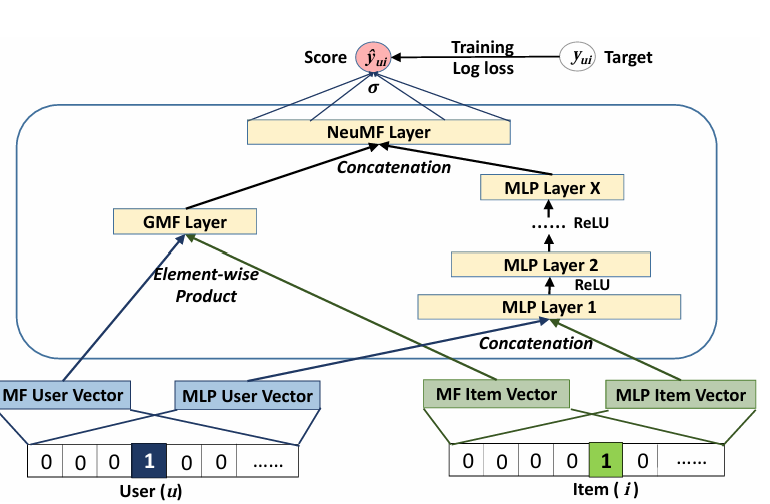
\includegraphics[width=0.5\linewidth]{diagram.png}
    \caption{Schematic illustration of the NeuMF architecture combining GMF and MLP.(Figure adapted from ~\cite{he2017neural}).}
    \label{fig:neumf-diagram}
\end{figure}

An additional design aspect of NeuMF is that it naturally accommodates both randomly initialized training and pretraining schemes. In the latter case, GMF and MLP can first be trained as standalone models, and their learned parameters used to initialize the corresponding branches of NeuMF. Let $\mathbf{h}^{\text{GMF}}$ and $\mathbf{h}^{\text{MLP}}$ denote the output-layer weight vectors learned separetely by GMF and MLP models, respectively. NeuMF interpolates between these two sets of weights using a balance parameter $\alpha \in [0,1]$ that controls the relative contribution of each branch:
\[
    \mathbf{h} \;\leftarrow\;
    \begin{bmatrix}
        \alpha \,\mathbf{h}^{\text{GMF}} \\
        (1 - \alpha)\,\mathbf{h}^{\text{MLP}}
    \end{bmatrix}.
\]
For $\alpha$ close to $1$, the prediction is dominated by the GMF branch; for $\alpha$ close to $0$, it is dominated by the MLP branch. This initialization strategy encourages NeuMF to inherit the strengths of both components while still allowing joint optimization of all parameters.

\subsubsection{ConvNCF}

Convolutional Neural Collaborative Filtering (ConvNCF) extends Neural Collaborative Filtering by replacing the vector-wise interaction function with a convolutional architecture operating on an outer-product interaction map~\cite{he2018convncf}. The main motivation to do that, is that outer-product should better cover the relationship between the embedded user and item vectors. Using the outer product, and pretraining we can build sort of a heat map \ref{fig:heat_map_movie}, which later can be passed through the convolutional neural network. At first glance, ConvNCF does not seem as a good fit for using it on user-item interaction data, However, the visible patterns might emerge after pre-training (see Figure \ref{fig:heat_map_movie}) might possibly suggest that the training process might learn spatial patterns in the data. This thesis answer the questions whether it is possible.
\begin{figure}[H]
    \centering
    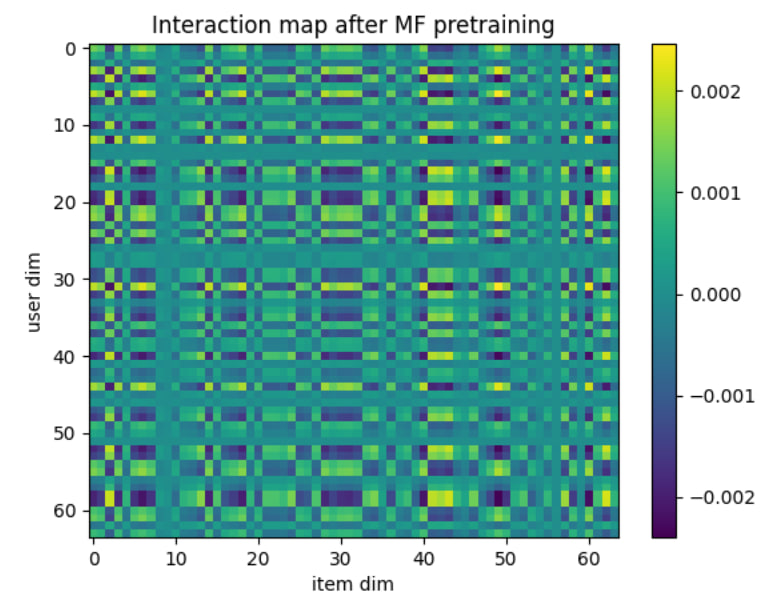
\includegraphics[width=0.5\linewidth]{image1000.png}
    \caption{Interaction map of emdeddings after Pretraining the MF model on MovieLens dataset}
    \label{fig:heat_map_movie}
\end{figure}

As in GMF and MLP, each user $u$ and item $i$ is first represented by $k$-dimensional latent embeddings $\mathbf{p}_u, \mathbf{q}_i \in \mathbb{R}^k$. Instead of combining these embeddings via an element-wise product or concatenation, ConvNCF constructs a two-dimensional interaction map using the outer product
\[
    \mathbf{E}_{ui} = \mathbf{p}_u \mathbf{q}_i^\top \in \mathbb{R}^{k \times k},
\]
where the $(s,t)$-th entry captures the interaction between the $s$-th latent dimension of the user and the $t$-th latent dimension of the item. This interaction map explicitly models pairwise correlations between latent dimensions, rather than aggregating them into a single scalar at the outset.

The interaction map $\mathbf{E}_{ui}$ is then normalized before being fed into the convolutional layers. This normalization step is not explicitly specified in the original ConvNCF paper~\cite{he2018convncf}, but in our experiments it proved important for stabilizing training.
The normalized interaction map is  processed by a stack of two-dimensional convolutional layers \ref{fig:convlayers}.
\begin{figure}[H]
    \centering
    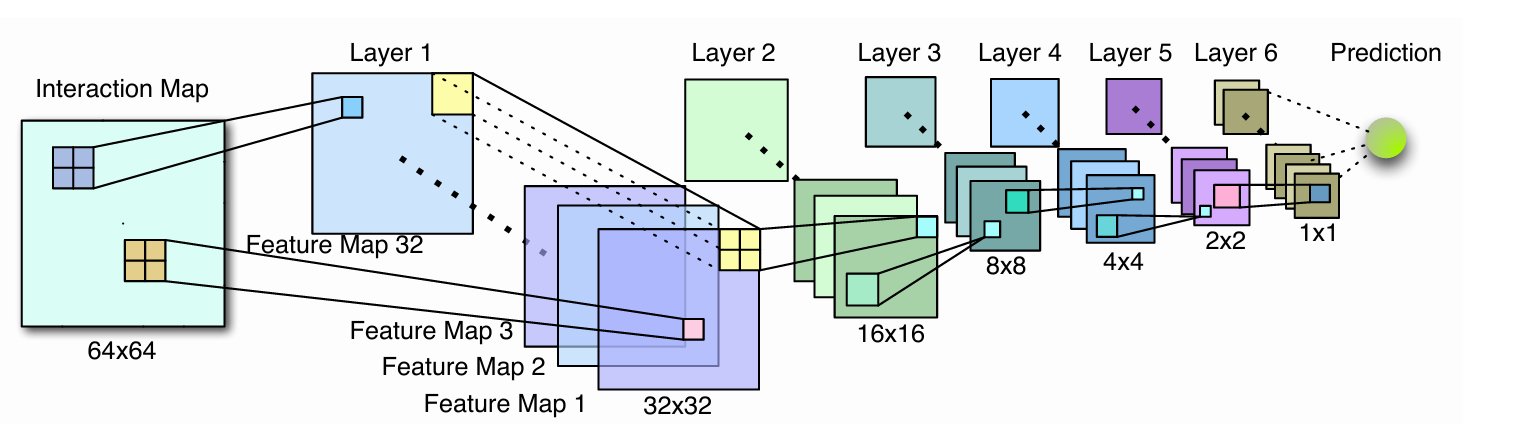
\includegraphics[width=0.7\linewidth]{conv.png}
    \caption{An example of the architecture of our ConvNCF model that has 6 convolution layers with embedding size 64 (Figure adapted from \cite{he2018convncf}).}
    \label{fig:convlayers}
\end{figure}

Let $\mathbf{E}_{ui}^{(0)} = \mathbf{E}_{ui}$ denote the input map, and let $\mathbf{E}_{ui}^{(\ell)}$ denote the feature maps at convolutional layer $\ell$. Each layer applies multiple learnable filters to the previous feature maps, followed by a non-linear activation
\[
    \mathbf{E}_{ui}^{(\ell)} = a_\ell \bigl( \mathrm{Conv2D}(\mathbf{E}_{ui}^{(\ell-1)}; \mathbf{W}_\ell, \mathbf{b}_\ell) \bigr),
\]
where $\mathbf{W}_\ell$ and $\mathbf{b}_\ell$ denote the convolutional kernels and biases at layer $\ell$, and $a_\ell(\cdot)$ is the activation function. In typical configurations, multiple convolutional stages are stacked, with the number of feature maps increasing in deeper layers to capture increasingly abstract interaction patterns.

After the final convolutional layer, the resulting feature maps are flattened into a vector $\mathbf{z}_{\text{conv}}$ and passed through a fully connected output layer with a sigmoid activation:
\[
    \hat{y}_{ui} = \sigma\!\bigl( \mathbf{h}^\top \mathbf{z}_{\text{conv}} \bigr),
\]
where $\mathbf{h}$ is the output weight vector and $\sigma(\cdot)$ is the logistic sigmoid function. This yields a predicted relevance score $\hat{y}_{ui} \in (0,1)$ for each user--item pair. By operating on the outer-product interaction map with convolutional filters, ConvNCF is suggested to be able to capture local patterns, if any, and higher-order dependencies among latent dimensions, going beyond the element-wise interactions of GMF and the vector-wise transformations of the MLP component.

In this thesis, a shallower ConvNCF variant is used compared to the original paper, with three convolutional layers having $\{32, 32, 64\}$ filters, respectively, and an embedding size of $k=64$.
    
\subsection{Bayesian Personalized Ranking loss}
In \cite{he2018convncf}, Bayesian Personalized Ranking (BPR) loss is used as the optimization objective. 
BPR was introduced by Rendle et al.~\cite{rendle2012bpr} specifically for implicit-feedback data, where 
only positive observations are available. Traditional pointwise losses treat observations as binary labels 
$(1/0$ for observed/unobserved$)$ and implicitly interpret all unobserved entries as negatives, which does 
not reflect relative preferences between items and can incorrectly suggest that $y_{ui} = 0$ means that 
user $u$ dislikes item $i$. BPR solves this by avoiding absolute labels. It only assumes:
\[
\text{if user clicked item } i \text{ but not item } j,\qquad i \succ j
\]

Specifically for recommendation systems we can implement the BPR in the following way:
The training process is performed over triplets $(u,i,j)$, where $i$ is an item with which user $u$ has an observed interaction ($y_{ui} = 1$), and $j$ is an item with which user $u$ has no observed interaction ($y_{uj} = 0$), sampled (uniform sampling) from the set of unobserved items. For a given model with predicted scores $\hat{y}_{ui}$ and $\hat{y}_{uj}$, BPR assumes that the user should prefer item $i$ over item $j$, and defines the objective in terms of the difference $\hat{y}_{ui} - \hat{y}_{uj}$. The BPR loss is given by
\[
    \mathcal{L}_{\text{BPR}}
    = - \sum_{(u,i,j) \in \mathcal{S}} 
      \ln \sigma\!\bigl( \hat{y}_{ui} - \hat{y}_{uj} \bigr)
      + \lambda \lVert \Theta \rVert_2^2,
\]
where $\mathcal{S}$ is the set of sampled triplets, $\Theta$ denotes all trainable model parameters, $\sigma(\cdot)$ is the sigmoid function, and $\lambda$ is a regularization coefficient. Minimizing $\mathcal{L}_{\text{BPR}}$ encourages the model to assign higher scores to observed items than to unobserved ones for each user.


\subsubsection{MF-BPR}

MF-BPR uses the same user and item embeddings as standard MF, but is trained with the pairwise BPR loss instead of a pointwise loss. The predicted score is still
\[
  \hat{y}_{ui} = \mathbf{p}_u^\top \mathbf{q}_i,
\]
but optimisation is performed over triplets $(u,i,j)$ with the BPR objective.


\subsection{Negative sampling strategy}

The models considered in this thesis are trained on implicit feedback data, where only positive user--item interactions are observed and all other entries in the interaction matrix are unobserved. In such settings, it is not appropriate to treat all unobserved pairs as true negatives, and training therefore relies on negative sampling to construct informative training instances from the space of unobserved user-item pairs.

Two types of objectives are employed. KNN is a memory-based method and does not optimize a loss function. The MF, GMF, MLP and NeuMF models are trained with a \emph{pointwise} loss, namely the binary cross-entropy between the predicted score $\hat{y}_{ui}$ and a binary target label $y_{ui} \in \{0,1\}$. For each observed interaction $(u,i)$ with $y_{ui}=1$, a fixed number of unobserved items $j$ is sampled for the same user and included as negative examples with label $y_{uj}=0$. In contrast, the MF-BPR and ConvNCF models are trained with the \emph{pairwise} BPR, where each training instance is a triplet $(u,i,j)$ encoding the preference of user $u$ for a positive item $i$ over a sampled negative item $j$.

To ensure a consistent training protocol across models, the same negative sampling rate is used throughout the experiments. For each positive interaction $(u,i)$ in the training data, four distinct negative items $j_1,\dots,j_4$ are sampled uniformly  from the set of items with which user $u$ has not interacted. This universal setting of \texttt{neg\_sample}~$=4$ is applied to all parameterized models, except ConvNCF. In the pointwise case (GMF, MLP, NeuMF), this yields one positive example and four negative examples per observed interaction. 
For MF-BPR and ConvNCF, we instead construct triplets $(u,i,j)$ for the BPR loss. MF-BPR uses four negatives per positive (four triplets), whereas on Yelp and for ConvNCF we set \texttt{num\_neg} = 1 to control training time, resulting in one triplet per positive interaction.



\subsection{Experimental setups}
\subsubsection{Evaluation Metrics}

To assess the quality of our recommender model, we adopt two widely used top-$K$ evaluation metrics: Hit Ratio (HR) and Normalized Discounted Cumulative Gain (NDCG) at cutoff $K$.

\noindent\textbf{Hit Ratio (HR@K)}\\
Measures whether the truth item appears among the top-$K$ recommendations:
\[
  \mathrm{HR@K}
  = \frac{1}{|U|} \sum_{u \in U}
    \mathbf{1}\bigl(i_u^+ \in \{i_{u,1}, \dots, i_{u,K}\}\bigr)
\]
where $U$ is the set of test users, $i_u^+$ is the held-out item for user $u$, and $\mathbf{1}(\cdot)$ is the indicator function.

\medskip
\noindent\textbf{Normalized Discounted Cumulative Gain (NDCG@K)}\\
Weights the hit by its position in the ranking:
\[
  \mathrm{NDCG@K}
  = \frac{1}{|U|} \sum_{u \in U}
    \sum_{p=1}^{K}
      \frac{\mathbf{1}(i_{u,p} = i_u^+)}{\log_2(p+1)}
\]
where $i_{u,p}$ is the item at rank $p$ for user $u$. A hit at position 1 contributes 1, at position 2 contributes $1/\log_2 3$, etc. Below in the table \ref{table:ndcg} weights for different positions are shown.

\begin{table}[H]
\centering
\begin{tabular}{c c c}
\hline
\textbf{Rank $p$} & \textbf{Discount Weight} & \textbf{Value} \\
\hline
1 & $\frac{1}{\log_2(p+1)}$ & $1$ \\
2 & $\frac{1}{\log_2 3}$ & $0.6309$ \\
3 & $\frac{1}{\log_2 4}$ & $0.5000$ \\
4 & $\frac{1}{\log_2 5}$ & $0.4307$ \\
5 & $\frac{1}{\log_2 6}$ & $0.3869$ \\
10 & $\frac{1}{\log_2 11}$ & $0.2891$ \\
20 & $\frac{1}{\log_2 21}$ & $0.2320$ \\
\hline
\end{tabular}
\caption{Discount weights used in NDCG@K. Higher ranks receive stronger reward.}
\label{table:ndcg}
\end{table}


\medskip
In the experiments, \emph{HR@10} and \emph{NDCG@10} are reported. For each user, a candidate set is constructed by taking the held-out positive item and augmenting it with a fixed number (99) of items that the user has not interacted with (treated as negatives). The resulting set of user-   item pairs is fed through the model to obtain predicted scores. The top K items according to these scores form the recommendation list for that user, and \emph{HR@K} and \emph{NDCG@K} are then computed on this list.

When comparing models or hyperparameter configurations, \emph{NDCG@10} serves as the primary selection criterion, as it accounts for the position of the correctly ranked item. In cases where two configurations achieve identical or nearly identical \emph{NDCG@10} values, we use \emph{HR@10} as a secondary tie-breaking metric.
\subsection{Hyperparameters}

To ensure a controlled comparison across architectures, a common hyperparameter configuration is adopted whenever possible. Unless stated otherwise, all trainable models are trained with:
\begin{itemize}
    \item mini-batch size $\texttt{batch\_size} = 256$;
    \item embedding dimension $\texttt{emb\_size} = 64$;
    \item a maximum of $30$ training epochs.
\end{itemize}
For model with relatively low computational cost (MF-BPR), the number of training epochs is increased to $50$ in order to give more opportunity for the model to converge. 

In all cases, model selection is based on validation performance: after every 3 epochs, \emph{NDCG@10} and \emph{HR@10} are evaluated on a validation split, and the checkpoint with the highest validation metrics is retained. This selected set of weights is then used for reporting final results (plots) and for the analysis of performance at different cut-off values $K$ for the test set (the $K$-analysis).
%%%check here::
Two dataset–model combinations deviate from the default hyperparameter settings due to stability considerations. For the ConvNCF model on the Yelp dataset, the negative sampling rate is reduced to $\texttt{num\_neg} = 1$ in order to control training time and memory consumption given the higher computational cost of the convolutional architecture. For ConvNCF on Yelp, a grid search is carried out over the $L_2$ regularization strength applied to the embedding and convolutional layers, with the learning rate fixed to $\eta = 0.05$ and optimization performed using the Adagrad algorithm with mini-batches. For NeuMF on Yelp, a grid search over the learning rate is performed while keeping the remaining hyperparameters fixed at their default values.

For every model, validation is carried out under the same leave-one-out protocol as used for training: the training interactions are further split into an internal training portion and a validation portion by holding out the most recent interaction per user from the training set. This internal validation split is used exclusively for hyperparameter tuning and for monitoring convergence, while the held-out test interactions remain untouched until the final evaluation.

\section{Results}



\subsection{KNN}

\subsubsection{MovieLens}
Table~\ref{tab:itemknn_movielens_results_topn200} reports the test performance of the ItemKNN best baseline on the MovieLens dataset for different recommendation cut-offs $K$, using a neighbourhood size of $\texttt{topN} = 200$. As expected, both \emph{HR@K} and \emph{NDCG@K} increase with larger cut-off values. Moving from $K=5$ to $K=20$ improves \emph{HR@K} from $0.3652$ to $0.7017$ and \emph{NDCG@K} from $0.2521$ to $0.3482$, indicating that the model retrieves a substantial fraction of relevant items when allowed a longer recommendation list.

\begin{table}[H]
\centering
\caption{ItemKNN Test Performance on the MovieLens Dataset (topN = 200)}
\label{tab:itemknn_movielens_results_topn200}
\begin{tabular}{c c c}
\hline
\textbf{K} & \textbf{HR@K} & \textbf{NDCG@K} \\
\hline
5  & 0.3652 & 0.2521 \\
10 & 0.5204 & 0.3022 \\
20 & 0.7017 & 0.3482 \\
\hline
\end{tabular}
\end{table}
The choice of neighbourhood size is visualized in the validation curves in Figure~\ref{fig:knn_movielens_val}. Validation \emph{HR@10} and \emph{NDCG@10} are relatively flat a wide range of neighbourhood sizes, with a slight improvement around $\texttt{topN} \approx 200$. This suggests that, for MovieLens, ItemKNN benefits from aggregating information from a moderately large set of neighbours, but the model is insensitive to further increases in neighbourhood size.



\begin{figure}[H]
    \centering
    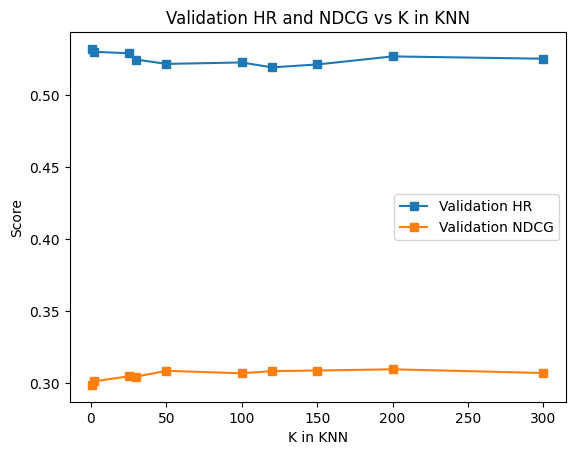
\includegraphics[width=0.5\linewidth]{image300.png}
    \caption{KNN Validation HR@10 and NDCG@10 on MovieLens dataset}
    \label{fig:knn_movielens_val}
\end{figure}

\subsubsection{Yelp}
Table~\ref{tab:itemknn_yelp_results_topn100} summarises the test performance of ItemKNN on the Yelp dataset for different cut-offs $K$, using a neighbourhood size of $\texttt{topN} = 100$. Compared to MovieLens, the scores are substantially higher across all cut-offs: for $K=10$, \emph{HR@10} reaches $0.7301$ and \emph{NDCG@10} reaches $0.4747$, and for $K=20$ the metrics further increase to $0.8461$ and $0.5050$, respectively. This indicates that on Yelp, the neighbourhood-based baseline is able to recover a large portion of users' held-out interactions.

However, we can clearly see a mismatch between HR@K and NDCG@K values, which means that KNN can indeed find the neighbor connections, but it cannot put the value on the connection, and determine which one is higher rated than others for a particular user.

\begin{table}[H]
\centering
\caption{ItemKNN Test Performance on the Yelp Dataset (topN = 100)}
\label{tab:itemknn_movielens_results}
\begin{tabular}{c c c}
\hline
\textbf{K} & \textbf{HR@K} & \textbf{NDCG@K} \\
\hline
5  & 0.5933 & 0.4320 \\
10 & 0.7301 & 0.4747 \\
20 & 0.8461 & 0.5050 \\
\hline
\end{tabular}
\end{table}
The corresponding validation curves in Figure~\ref{fig:knn_yelp_val} show that \emph{HR@10} and \emph{NDCG@10} increase rapidly when the neighbourhood size grows from very small values and then plateau once $\texttt{topN}$ reaches approximately $50$–$100$. Beyond this point, additional neighbours yield only marginal gains. In combination with the test results, this pattern suggests that Yelp exhibits stronger and more consistent close-by neighbourhood structure than MovieLens.


\begin{figure}[H]
    \centering
    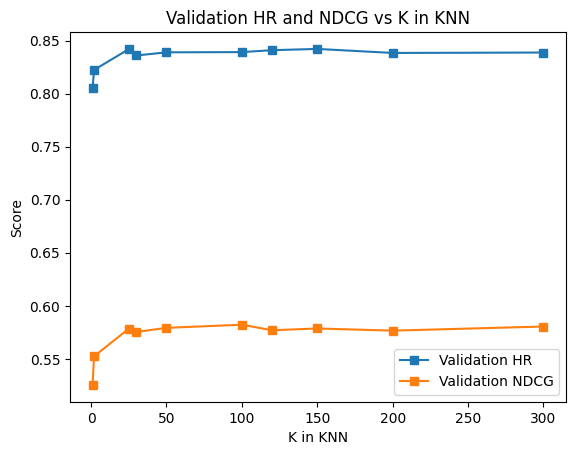
\includegraphics[width=0.5\linewidth]{image301.png}
    \caption{KNN Validation HR@10 and NDCG@10 on Yelp dataset}
    \label{fig:knn_yelp_val}
\end{figure}

\subsection{MF BPR}

Table~\ref{tab:mfbpr_movielens_results} reports the top-$K$ test performance of the MF-BPR model on the MovieLens dataset. As $K$ increases from $5$ to $20$, both \emph{HR@K} and \emph{NDCG@K} improve substantially: \emph{HR@K} rises from $0.3634$ to $0.7300$, while \emph{NDCG@K} increases from $0.2409$ to $0.3460$. This indicates that MF-BPR is able to retrieve a sizable fraction of relevant items when allowed a moderately long recommendation list.

\subsubsection{MovieLens}
\begin{table}[H]
\centering
\caption{MF-BPR Test Performance on the MovieLens Dataset (epoch = 50)}
\label{tab:mfbpr_movielens_results}
\begin{tabular}{c c c}
\hline
\textbf{K} & \textbf{HR@K} & \textbf{NDCG@K} \\
\hline
5  & 0.3634 & 0.2409 \\
10 & 0.5379 & 0.2989 \\
20 & 0.7300 & 0.3460 \\
\hline
\end{tabular}
\end{table}
The training dynamics on MovieLens are shown in Figures~\ref{fig:mfbpr_movielens_train} and~\ref{fig:mfbpr_movielens_val}. The training loss decreases steadily while the training accuracy (the proportion of correctly ordered positive-negative pairs under the BPR objective) increases and quickly plateaus at a high level. On the validation set, both \emph{HR@10} and \emph{NDCG@10} improve sharply in the early epochs and then continue to grow more gradually, suggesting that the model is on the way to converge without clear signs of overfitting within the chosen number of epochs (50). The training was stopped due to long computing time of running it for 50 epochs. 

\begin{figure}[H]
    \centering
    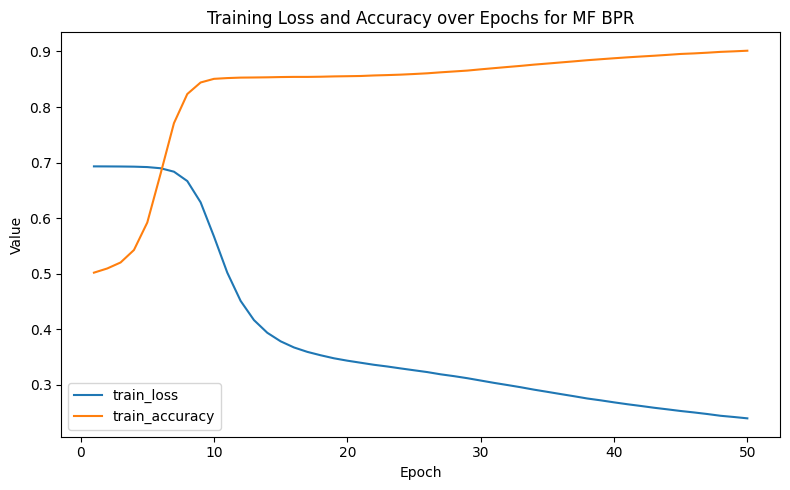
\includegraphics[width=0.5\linewidth]{image121.png}
    \caption{MF BPR training loss and training accuracy over 50 epochs on MovieLens dataset}
    \label{fig:mfbpr_movielens_train}
\end{figure}
\begin{figure}[H]
    \centering
    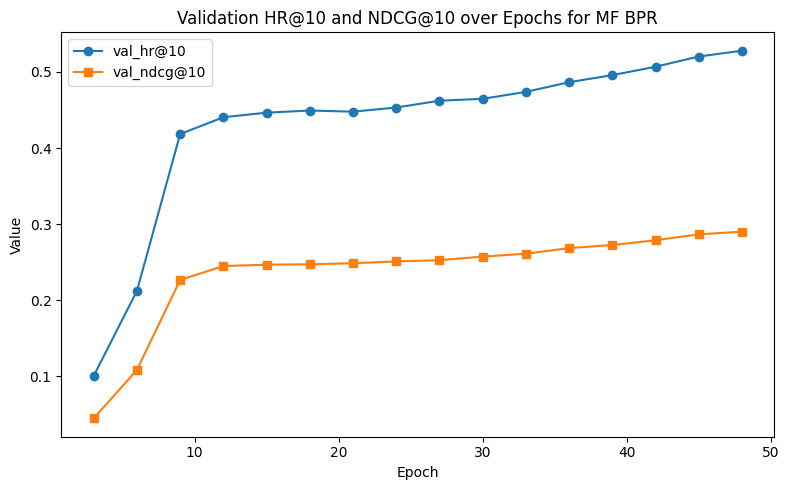
\includegraphics[width=0.5\linewidth]{image122.png}
    \caption{MF BPR validation HR@10 and NDCG@10 over 50 epochs (every 3 epochs) on MovieLens dataset}
    \label{fig:mfbpr_movielens_val}
\end{figure}
\subsubsection{Yelp}
Table~\ref{tab:mfbpr_yelp_results} presents the corresponding MF-BPR results on the Yelp dataset. The absolute scores are lower than on MovieLens, reflecting the higher sparsity and noisier interactions in Yelp. Nevertheless, the same monotonic trend with respect to $K$ is observed: \emph{HR@K} increases from $0.3235$ at $K=5$ to $0.5572$ at $K=20$, and \emph{NDCG@K} increases from $0.2296$ to $0.2958$. Thus, MF-BPR is still able to learn a meaningful portion of users' held-out items, although worse than for denser MovieLens setting.

\begin{table}[H]
\centering
\caption{MF-BPR Test Performance on the Yelp Dataset  (epoch = 50)}
\label{tab:mfbpr_yelp_results}
\begin{tabular}{c c c}
\hline
\textbf{K} & \textbf{HR@K} & \textbf{NDCG@K} \\
\hline
5  & 0.3235 & 0.2296 \\
10 & 0.4329 & 0.2666 \\
20 & 0.5572 & 0.2958 \\
\hline
\end{tabular}
\end{table}
Figures~\ref{fig:mfbpr_yelp_train} and~\ref{fig:mfbpr_yelp_val} illustrate the learning behavior on Yelp. Training accuracy increases steadily throughout training, while the loss remains relatively stable and then starts to decrease, indicating that the pairwise ranking objective becomes progressively better satisfied. On the validation data, both \emph{HR@10} and \emph{NDCG@10} exhibit a consistent upward trend, with particularly strong gains in later epochs. This suggests that MF-BPR benefits from longer training on the sparser Yelp dataset, and that the model is, once again on its way to convergence.

\begin{figure}[H]
    \centering
    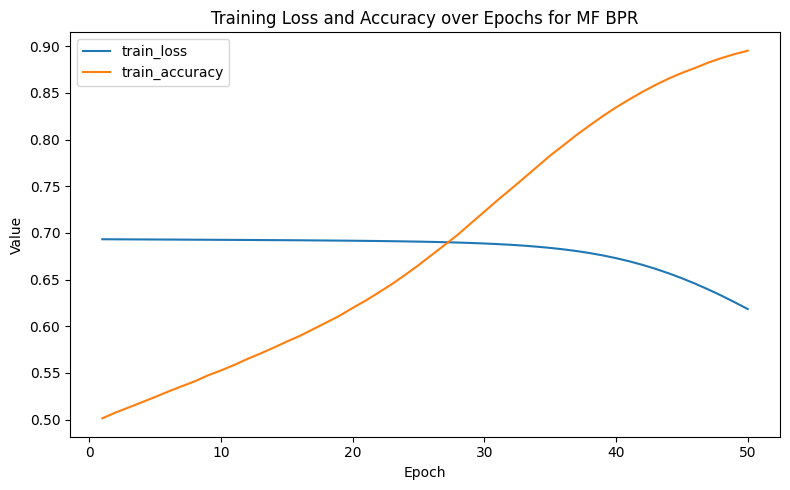
\includegraphics[width=0.5\linewidth]{image130.png}
    \caption{MF BPR training loss and training accuracy over 50 epochs on Yelp dataset}
    \label{fig:mfbpr_yelp_train}
\end{figure}
\begin{figure}[H]
    \centering
    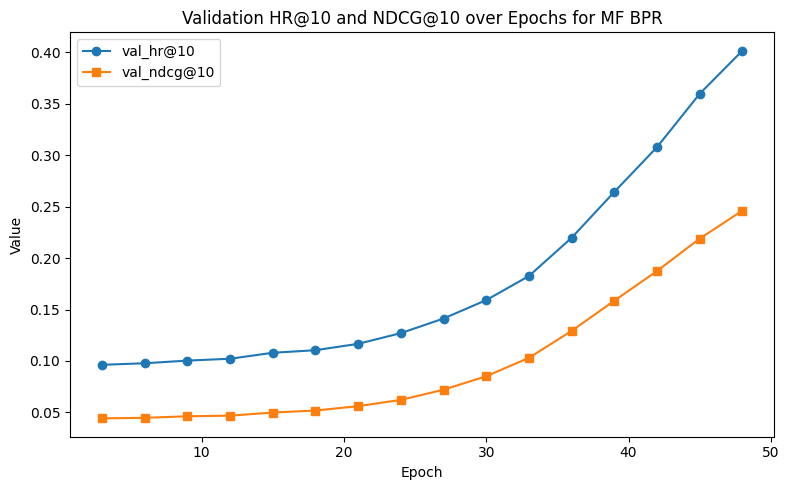
\includegraphics[width=0.5\linewidth]{image131.png}
    \caption{MF BPR validation HR@10 and NDCG@10 over 50 epochs (every 3 epochs) on MovieLens dataset}
    \label{fig:mfbpr_yelp_val}
\end{figure}



\subsection{GMF}
Table~\ref{tab:gmf_results} reports the test performance of GMF on the MovieLens dataset, evaluated at the epoch that achieves the best validation \emph{NDCG@10} (epoch~3). At this checkpoint, GMF attains \emph{HR@10} of $0.6629$ and \emph{NDCG@10} of $0.3853$, clearly outperforming the MF-BPR baseline and the KNN model at the same cut-off. As $K$ increases from $5$ to $20$, both metrics improve monotonically, with \emph{HR@K} rising from $0.4758$ to $0.8192$ and \emph{NDCG@K} from $0.3239$ to $0.4279$, indicating that GMF ranks really well top items for $K=20$.

\subsubsection{MovieLens}
\begin{table}[H]
\centering
\caption{GMF Test Performance at Best Epoch (Epoch 3) on MovieLens}
\label{tab:gmf_results}
\begin{tabular}{c c c}
\hline
\textbf{K} & \textbf{HR@K} & \textbf{NDCG@K} \\
\hline
5  & 0.4758 & 0.3239 \\
10 & 0.6629 & 0.3853 \\
20 & 0.8192 & 0.4279 \\
\hline
\end{tabular}
\end{table}
The training curves in Figure~\ref{fig:gmf_movielens_train} show that the training loss decreases rapidly and the  training accuracy quickly approaches $0.9$, after which both curves flatten. In contrast, the validation metrics in Figure~\ref{fig:gmf_movielens_val} exhibit the opposite behaviour: \emph{HR@10} and \emph{NDCG@10} are highest at the very beginning of training and then decline steadily over subsequent epochs. This pattern is a definite indication of overfitting: GMF continues to optimize the training objective while its generalisation performance worsens. For this reason, early stopping at epoch~3 is adopted (best \emph{NDCG}@10 value), and all MovieLens GMF results are reported from this checkpoint.

\begin{figure}[H]
    \centering
    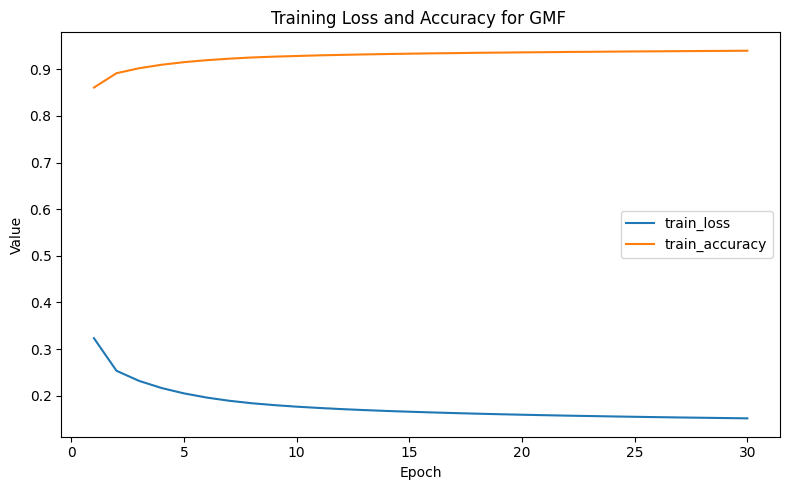
\includegraphics[width=0.5\linewidth]{image104.png}
    \caption{GMF training loss and training accuracy over 30 epochs on MovieLens dataset}
    \label{fig:gmf_movielens_train}
\end{figure}

\begin{figure}[H]
    \centering
    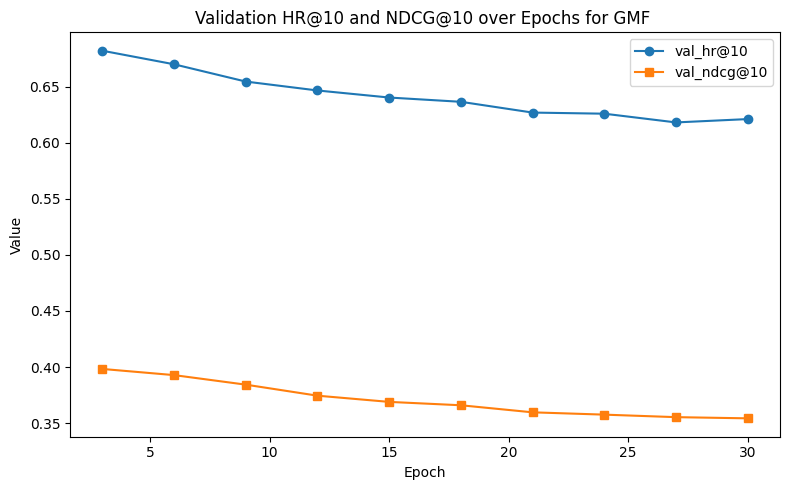
\includegraphics[width=0.5\linewidth]{image105.png}
    \caption{GMF validation HR@10 and NDCG@10 over 30 epochs (every 3 epochs) on MovieLens dataset}
    \label{fig:gmf_movielens_val}
\end{figure}
\subsubsection{Yelp}
Table~\ref{tab:gmf_yelp_results} presents the corresponding GMF performance on the Yelp dataset, again evaluated at the best validation epoch (epoch~3). At $K=10$, GMF achieves \emph{HR@10} of $0.6775$ and \emph{NDCG@10} of $0.4284$, however GMF is clearly worse than the ItemKNN baseline on Yelp, which suggests that local neighbourhood structure is particularly strong in this dataset. As on MovieLens, performance improves consistently with larger $K$, reaching \emph{HR@20} of $0.8039$ and \emph{NDCG@20} of $0.4578$.

\begin{table}[H]
\centering
\caption{GMF Test Performance on the Yelp Dataset at Best Epoch (Epoch 3)}
\label{tab:gmf_yelp_results}
\begin{tabular}{c c c}
\hline
\textbf{K} & \textbf{HR@K} & \textbf{NDCG@K} \\
\hline
5  & 0.5345 & 0.3800 \\
10 & 0.6775 & 0.4284 \\
20 & 0.8039 & 0.4578 \\
\hline
\end{tabular}
\end{table}

The training behaviour on Yelp, shown in Figure~\ref{fig:gmf_yelp_train}, is even more extreme: the training loss approaches zero and the training accuracy moves very close to $1.0$ within a few epochs. At the same time, the validation curves in Figure~\ref{fig:gmf_yelp_val} mirror the MovieLens case: both \emph{HR@10} and \emph{NDCG@10} are highest in the early epochs and then decrease monotonically. This again signals strong overfitting of GMF.  



\begin{figure}[H]
    \centering
    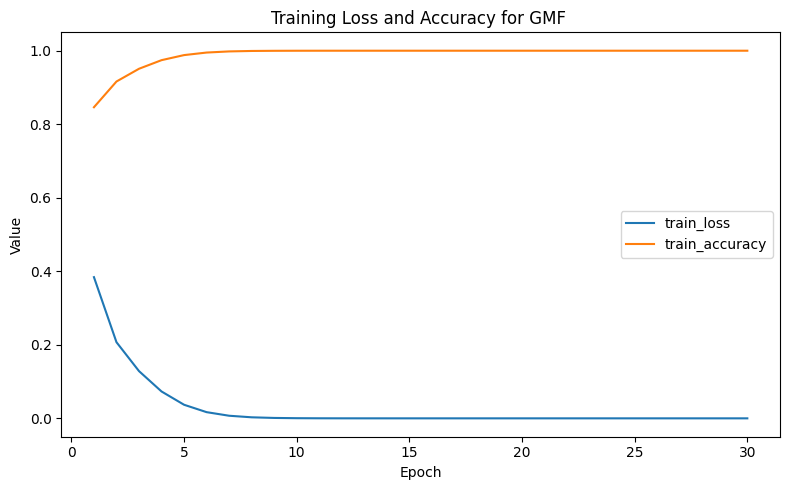
\includegraphics[width=0.5\linewidth]{image106.png}
    \caption{GMF training loss and training accuracy over 30 epochs on Yelp dataset}
    \label{fig:gmf_yelp_train}
\end{figure}

\begin{figure}[H]
    \centering
    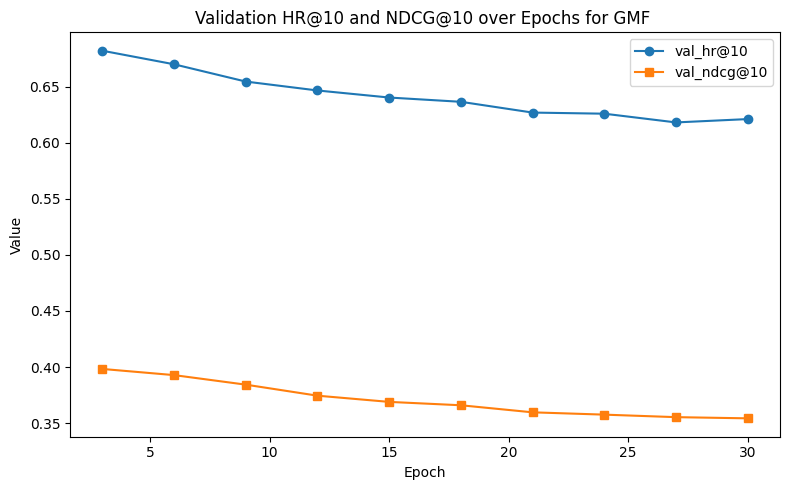
\includegraphics[width=0.5\linewidth]{image107.png}
    \caption{GMF validation HR@10 and NDCG@10 over 30 epochs (every 3 epochs) on Yelp dataset}
    \label{fig:gmf_yelp_val}
\end{figure}
Overall, GMF is capable of achieving good top-$K$ accuracy on both datasets, but the learning and validation curves highlight that, without a complex hyperparameter search, the model is overfitting early, thus has to be controlled via validation-based early stopping.
\subsection{MLP}

\subsubsection{MovieLens}
Table~\ref{tab:mlp_movielens_results} reports the test performance of the MLP model on the MovieLens dataset, evaluated at epoch 12. At this checkpoint the model attains on the test set \emph{HR@10} of $0.6358$ and \emph{NDCG@10} of $0.3675$, which is substantially higher than the MF-BPR  and slightly below the corresponding GMF scores. As $K$ increases, both metrics improve monotonically: \emph{HR@K} increases from $0.4568$ at $K=5$ to $0.8053$ at $K=20$, while \emph{NDCG@K} rises from $0.3078$ to $0.4115$. 

\begin{table}[H]
\centering
\caption{MLP Test Performance on the MovieLens Dataset at Best Epoch (Epoch 12)}
\label{tab:mlp_movielens_results}
\begin{tabular}{c c c}
\hline
\textbf{K} & \textbf{HR@K} & \textbf{NDCG@K} \\
\hline
5  & 0.4568 & 0.3078 \\
10 & 0.6358 & 0.3675 \\
20 & 0.8053 & 0.4115 \\
\hline
\end{tabular}
\end{table}
The training behaviour on MovieLens is shown in Figures~\ref{fig:mlp_movielens_train} and~\ref{fig:mlp_movielens_val}. The training loss decreases smoothly over epochs, while the  training accuracy increases and quickly stabilises close to $0.9$. On the validation set, \emph{HR@10} and \emph{NDCG@10} rise in the first few epochs, peak around epochs 9-12, and then remain almost flat with a slight downward trend. This pattern suggests mild overfitting: the model continues to learn the training data slightly better, but further this yields only marginal or negative impact on the validation performance. Consequently, early stopping at epoch 12 is adopted for reporting MovieLens MLP results.

\begin{figure}[H]
    \centering
    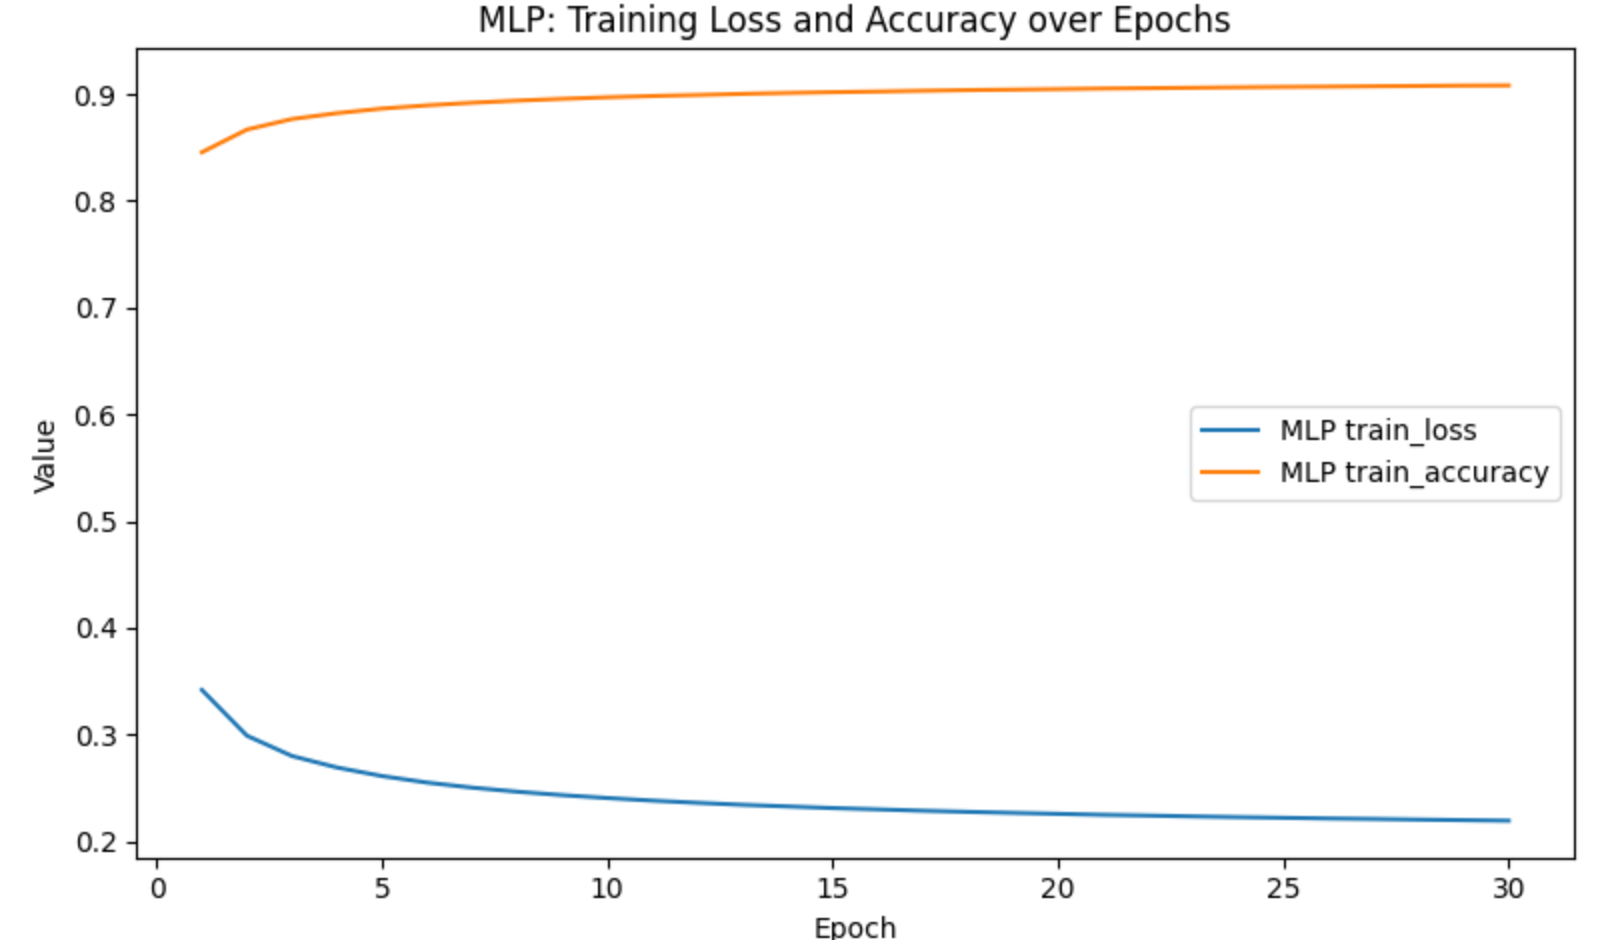
\includegraphics[width=0.5\linewidth]{image108.png}
    \caption{MLP training loss and training accuracy over 30 epochs on MovieLens dataset}
    \label{fig:mlp_movielens_train}
\end{figure}

\begin{figure}[H]
    \centering
    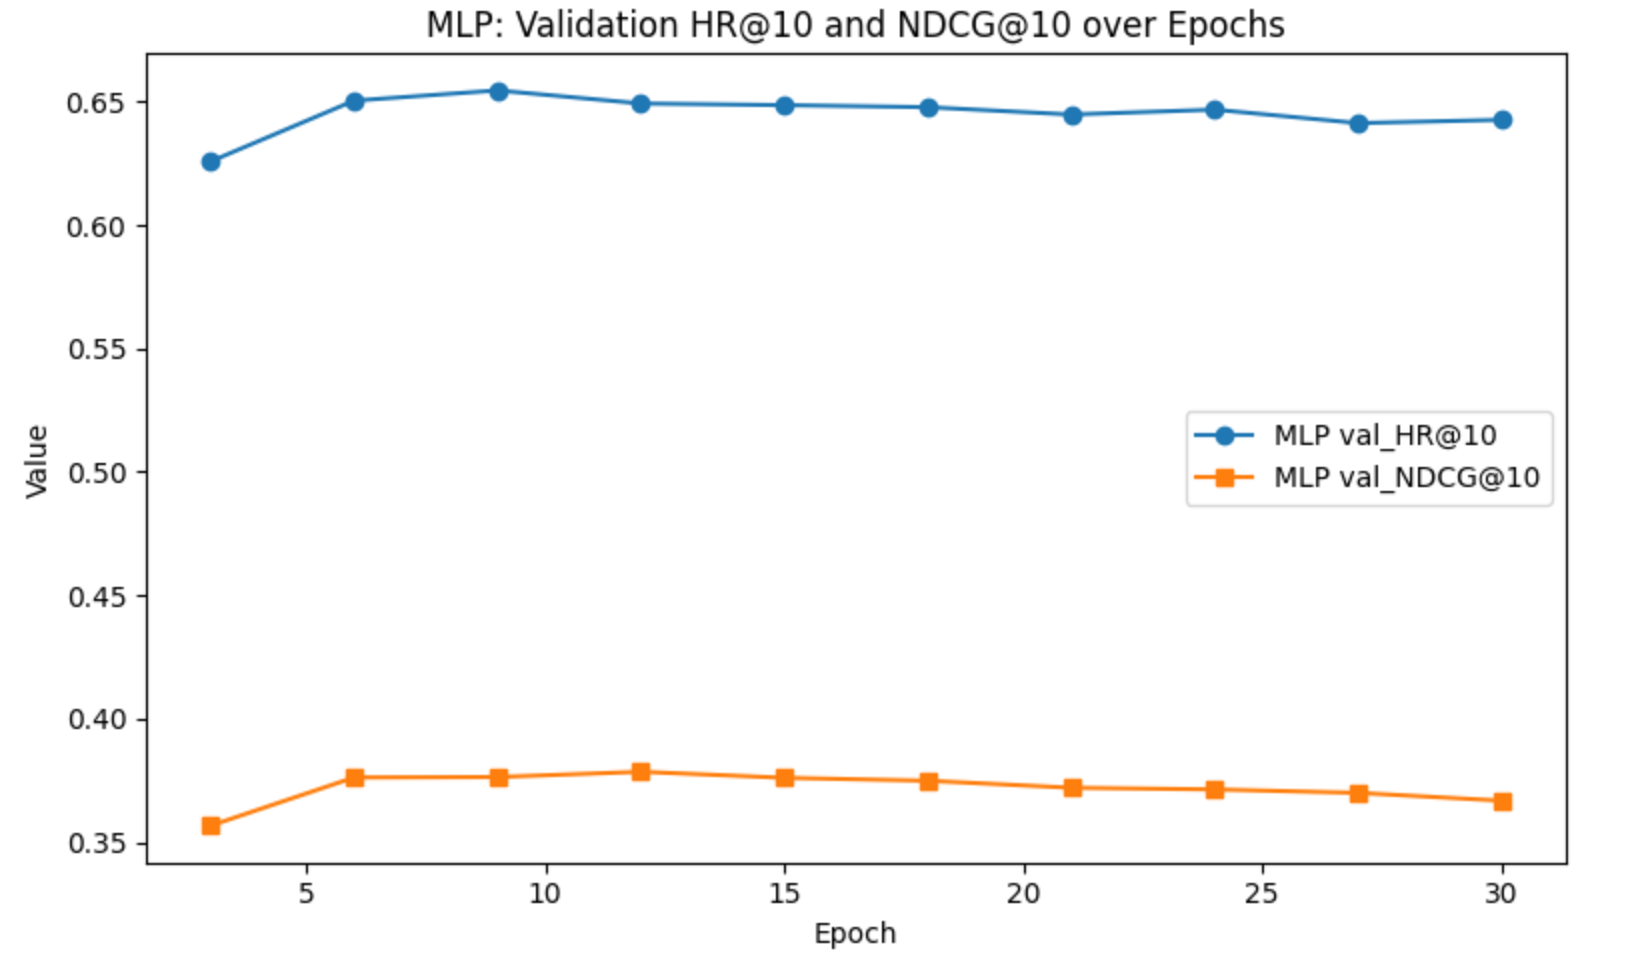
\includegraphics[width=0.5\linewidth]{image109.png}
    \caption{MLP validation HR@10 and NDCG@10 over 30 epochs (every 3 epochs) on MovieLens dataset}
    \label{fig:mlp_movielens_val}
\end{figure}

\subsubsection{Yelp}
Table~\ref{tab:mlp_yelp_results} shows the MLP performance on the Yelp dataset, evaluated at the best validation epoch (epoch 6). At $K=10$, the model achieves \emph{HR@10} of $0.6787$ and \emph{NDCG@10} of $0.4224$, which is competitive with GMF (slightly higher HR, but slightly lower NDCG). As on MovieLens, the performance increases with larger $K$, reaching \emph{HR@20} of $0.8162$ and \emph{NDCG@20} of $0.4558$.

\begin{table}[H]
\centering
\caption{MLP Test Performance on the Yelp Dataset at Best Epoch (Epoch 6)}
\label{tab:mlp_yelp_results}
\begin{tabular}{c c c}
\hline
\textbf{K} & \textbf{HR@K} & \textbf{NDCG@K} \\
\hline
5  & 0.5195 & 0.3688 \\
10 & 0.6787 & 0.4224 \\
20 & 0.8162 & 0.4558 \\
\hline
\end{tabular}
\end{table}
The learning curves in Figures~\ref{fig:mlp_yelp_train} and~\ref{fig:mlp_yelp_val} reveal a stronger form of overfitting on Yelp. The training loss steadily decreases towards zero and the training accuracy approaches $1.0$, indicating that the network almost perfectly satisfies the pairwise ranking constraints on the training set. In contrast, the validation metrics peak very early: both \emph{HR@10} and \emph{NDCG@10} reach their maximum around epoch 6 and then decline monotonically. Continuing training beyond this point would therefore harm generalisation. Early stopping at epoch 6 mitigates this effect and is used for all reported Yelp MLP results. As with GMF, these curves suggest that the MLP has more capacity than strictly necessary for the Yelp data and that stronger regularisation or a smaller architecture could further improve robustness.

\begin{figure}[H]
    \centering
    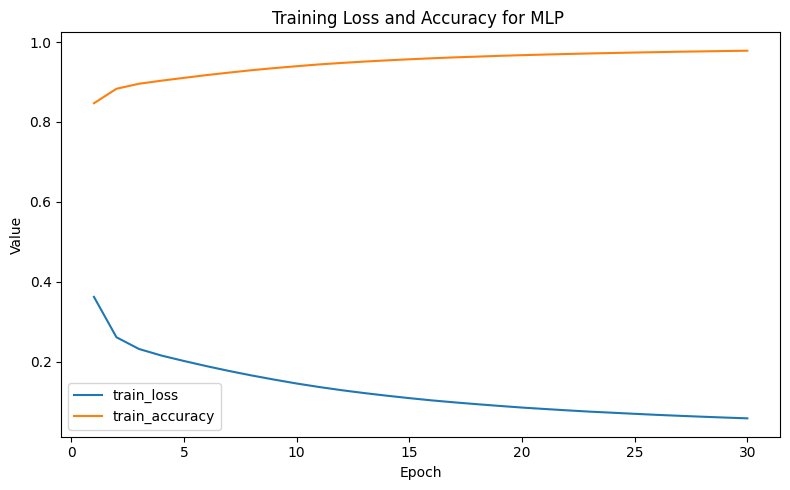
\includegraphics[width=0.5\linewidth]{image111.png}
    \caption{MLP training loss and training accuracy over 30 epochs on Yelp dataset}
    \label{fig:mlp_yelp_train}
\end{figure}

\begin{figure}[H]
    \centering
    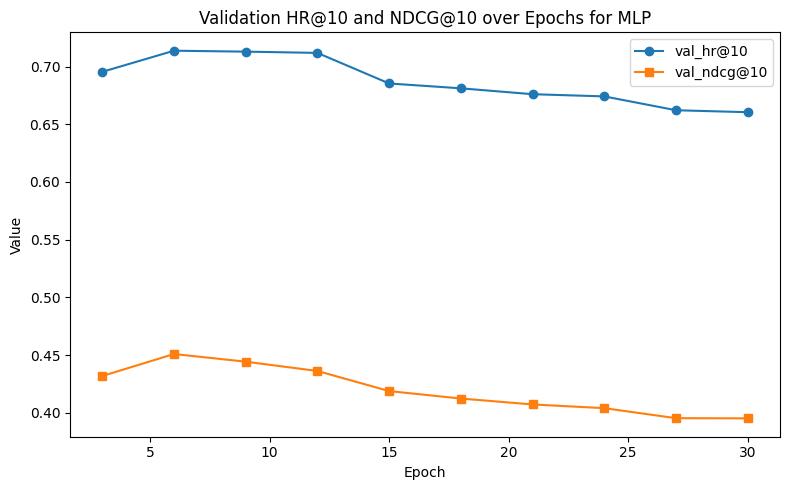
\includegraphics[width=0.5\linewidth]{image112.png}
    \caption{MLP validation HR@10 and NDCG@10 over 30 epochs (every 3 epochs) on Yelp dataset}
    \label{fig:mlp_yelp_val}
\end{figure}



%%%%%%%%%%%%%%%%%%%%%%%%%%%%%%%%%%%%%%%%%%%
%%%%%%%%%%%%%%%%%%%%%%%%%%%%%%%%%%%%%%%%%%%

\subsection{NeuMF wo pretraining}

%%%%%%%%%%%%%%%%%%%%%%%%%%%%%%%%%%%%%%%%%%%

\subsubsection{MovieLens}
Table~\ref{tab:neumf_movielens_results} reports the test performance of NeuMF (without pretraining) on the MovieLens dataset, evaluated at the epoch that yields the best validation values (epoch 3). At this epoch, NeuMF scores on the test set \emph{HR@10} of $0.6457$ and \emph{NDCG@10} of $0.3752$, which is slightly higher than MF-BPR and MLP, but marginally below GMF. As $K$ increases from $5$ to $20$, both metrics increase monotonically: \emph{HR@K} rises from $0.4684$ to $0.8103$, and \emph{NDCG@K} from $0.3170$ to $0.4158$.
\begin{table}[H]
\centering
\caption{NeuMF Test Performance on the MovieLens Dataset at Best Epoch (Epoch 3)}
\label{tab:neumf_movielens_results}
\begin{tabular}{c c c}
\hline
\textbf{K} & \textbf{HR@K} & \textbf{NDCG@K} \\
\hline
5  & 0.4684 & 0.3170 \\
10 & 0.6457 & 0.3752 \\
20 & 0.8103 & 0.4158 \\
\hline
\end{tabular}
\end{table}
The training curves in Figure~\ref{fig:neumf_movielens_train} show the now familiar pattern: the training loss decreases steadily and the pairwise training accuracy approaches a high value, indicating that the model fits the training data very well. In contrast, the validation metrics in Figure~\ref{fig:neumf_movielens_val} peak at the very beginning of training and then decline monotonically. Both \emph{HR@10} and \emph{NDCG@10} are highest around epoch~3 and deteriorate afterwards, which is a clear sign of overfitting. For this reason, early stopping at epoch~3 is applied, and all MovieLens NeuMF (without pretraining) results are reported from this checkpoint. 

Overall, NeuMF without pretraining does not produce a large gain over the simpler GMF on MovieLens, suggesting that the additional capacity in the MLP branch is mainly used to fit noise rather than to capture additional signal in this relatively dense dataset.

\begin{figure}[H]
    \centering
    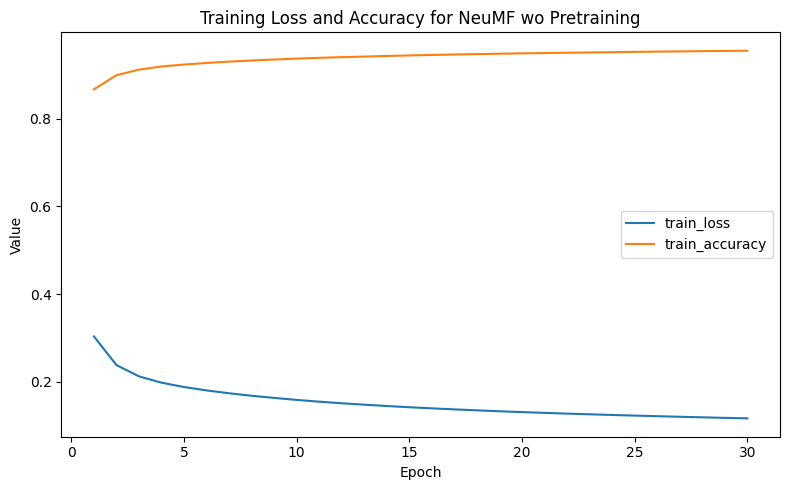
\includegraphics[width=0.5\linewidth]{image102.png}
 \caption{NeuMF training loss and training accuracy over 30 epochs on MovieLens dataset}
    \label{fig:neumf_movielens_train}
\end{figure}

\begin{figure}[H]
    \centering
    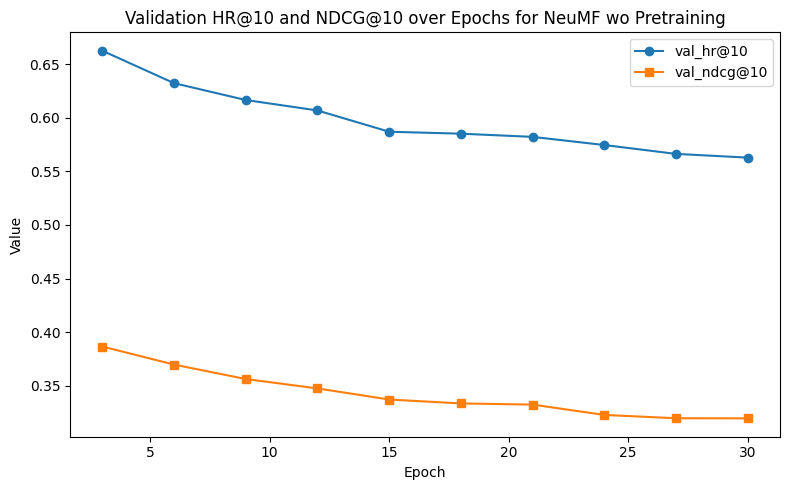
\includegraphics[width=0.5\linewidth]{image103.png}
    \caption{NeuMF validation HR@10 and NDCG@10 over 30 epochs (every 3 epochs) on MovieLens dataset}
    \label{fig:neumf_movielens_val}
\end{figure}
%%%%%%%%%%%%%%%%%%%%%%%%%%%%%%%%%%%%%%%%%%%

\subsubsection{Yelp}
Table~\ref{tab:neumf_yelp_results} summarises the NeuMF (without pretraining) results on the Yelp dataset, again evaluated at the best validation epoch (epoch~3). At $K=10$, the model achieves \emph{HR@10} of $0.6744$ and \emph{NDCG@10} of $0.4264$, which is very close to the corresponding GMF and MLP scores. As for MovieLens, performance increases with larger cut-off $K$, reaching \emph{HR@20} of $0.7919$ and \emph{NDCG@20} of $0.4555$.

\begin{table}[H]
\centering
\caption{NeuMF Test Performance on the Yelp Dataset at Best Epoch (Epoch 3)}
\label{tab:neumf_yelp_results}
\begin{tabular}{c c c}
\hline
\textbf{K} & \textbf{HR@K} & \textbf{NDCG@K} \\
\hline
5  & 0.5371 & 0.3794 \\
10 & 0.6744 & 0.4264 \\
20 & 0.7919 & 0.4555 \\
\hline
\end{tabular}
\end{table}
The training curves for Yelp, shown in Figure~\ref{fig:neumf_wo_pre_loss}, exhibit a slightly softer overfitting than on MovieLens: the training loss  approaches zero and the training accuracy converges to almost $1.0$ within 6-9 epochs, while validation curves (Figure~\ref{fig:neumf_wo_pre_metric}), grow towards for the first 6-9 epochs, and then steadily decrease.

Taken together, NeuMF without pretraining yields competitive results on both datasets but does not clearly outperform GMF or MLP given the chosen hyperparameters. The learning curves suggest that the model capacity is high relative to the amount of signal in the data, and that effective regularisation and early stopping are necessary to prevent overfitting.

\begin{figure}[H]
    \centering
    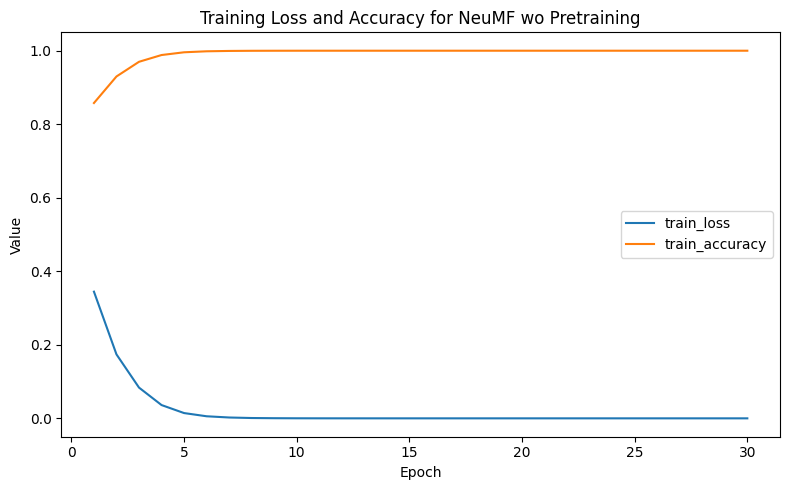
\includegraphics[width=0.5\linewidth]{image100.png}
    \caption{NeuMF training loss and training accuracy over 30 epochs on Yelp dataset}
    \label{fig:neumf_wo_pre_loss}
\end{figure}

\begin{figure}[H]
    \centering
    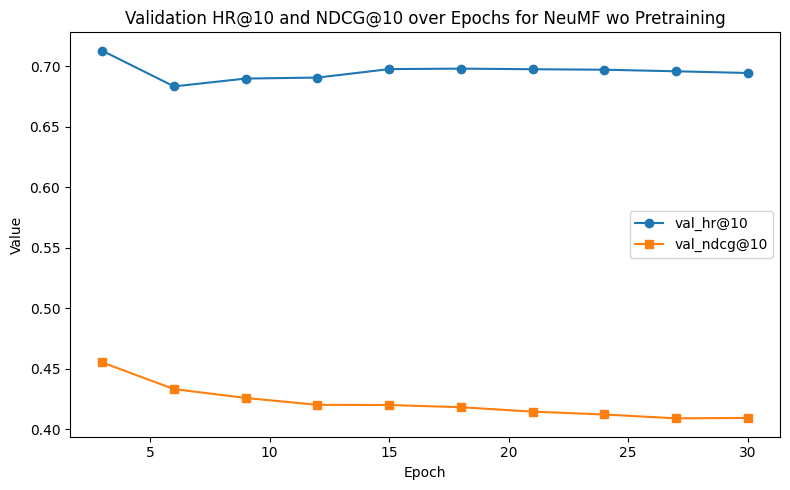
\includegraphics[width=0.5\linewidth]{image101.png}
    \caption{NeuMF validation HR@10 and NDCG@10 over 30 epochs (every 3 epochs) on Yelp dataset}
    \label{fig:neumf_wo_pre_metric}
\end{figure}

\subsection{Shallow ConvNCF}

\subsubsection{MovieLens}
The ConvNCF models $\ell2$ regulazation
$(\ell2\_emb , \ell2\_conv, \ell2\_out \in \{10^{-3}, 10^{-1}, 0\})$, where the $\ell2$ regularizes are for embedding layer, CNN layer, output layer, respectively. Parameters were tuned using a grid search, for most of the cases, the model exhibited inability to decrease the loss or to increase the pairwise accuracy. Nevertheless, for small $e\ell2$ values, there were signs of learning.

The ConvNCF results on MovieLens show that the model struggles to generalize despite almost perfect loss and pairwise accuracy on the training data.
Table~\ref{tab:convncf_movielens_results} reports the test performance at the epoch that achieves the highest validation \emph{NDCG@10} (epoch 15). At this checkpoint ConvNCF attains \emph{HR@10} of only $0.3220$ and \emph{NDCG@10} of $0.1606$, with \emph{HR@20} and \emph{NDCG@20} reaching $0.5040$ and $0.2071$, respectively. All these values are substantially below those of the MF-based and NeuMF models on MovieLens, indicating that the convolution outer-product architecture does not translate into improved ranking quality. Which indicates, that the model just "remembers the data", using its generalization abilities as a deep learning model, not learning the actual relationships in the data.
\begin{table}[H]
\centering
\caption{ConvNCF Test Performance on the MovieLens Dataset at Best Epoch 15}
\label{tab:convncf_movielens_results}
\begin{tabular}{c c c}
\hline
\textbf{K} & \textbf{HR@K} & \textbf{NDCG@K} \\
\hline
5  & 0.1838 & 0.1163 \\
10 & 0.3220 & 0.1606 \\
20 & 0.5040 & 0.2071 \\
\hline
\end{tabular}
\end{table}

The training curves in \ref{convncf_movielens_train} reveal extremely fast optimisation: the BPR loss collapses within a few epochs and the pairwise training accuracy rises to almost $1.0$, after which both curves remain flat. This shows that ConvNCF is able to fit the sampled training triplets almost perfectly. However, the validation metrics in \ref{convncf_movielens_val} tell a different story. Both \emph{HR@10} and \emph{NDCG@10} remain low overall and exhibit strong fluctuations across epochs, with sharp spikes around epochs 15 and 21 rather than a smooth upward trend. Such behavior is characteristic of problems with actually learning the data, and instead the model is memorizing the noise.



\begin{figure}[H]
    \centering
    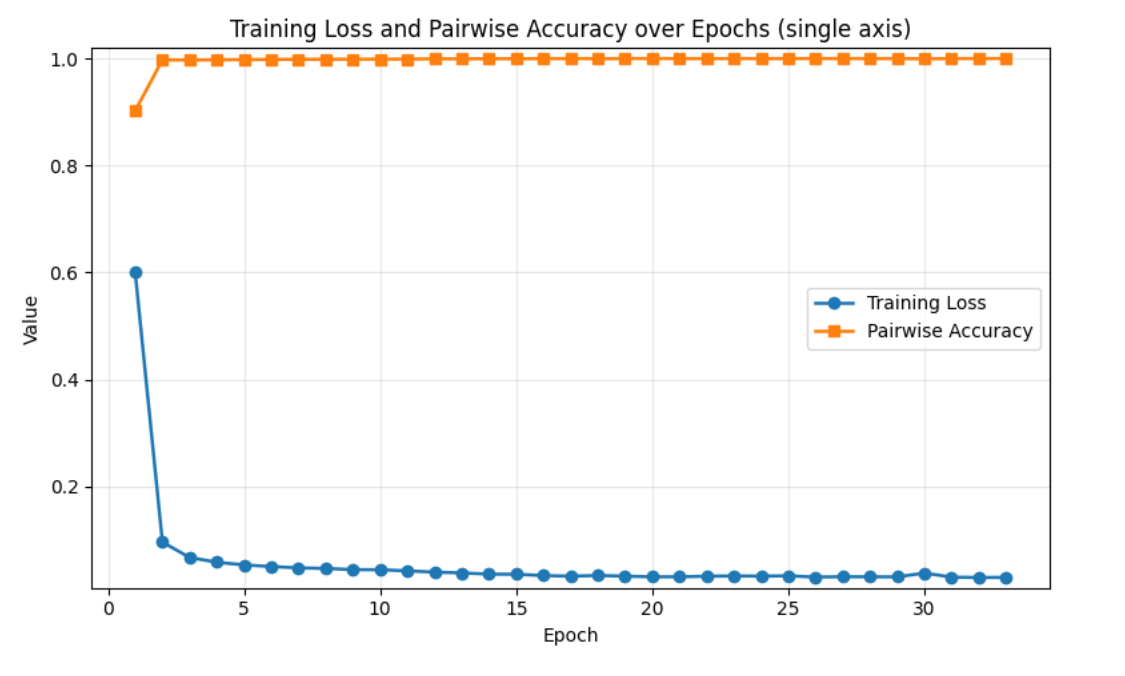
\includegraphics[width=0.5\linewidth]{image2.png}
       \caption{ConvNCF training loss and training accuracy over 30 epochs on MovieLens dataset}
       \label{fig:convncf_movielens_train}
\end{figure}
\begin{figure}[H]
    \centering
    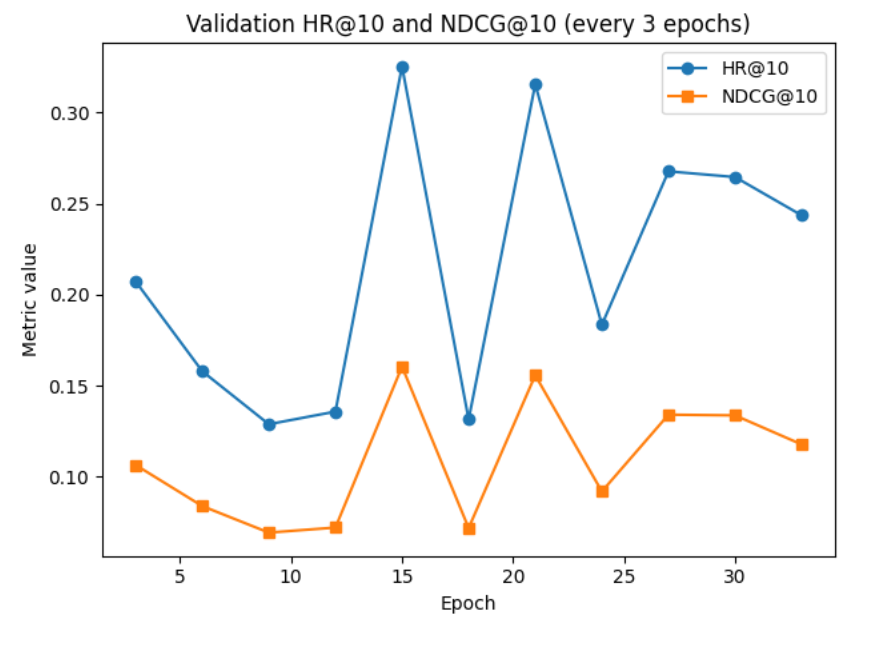
\includegraphics[width=0.5\linewidth]{image1.png}
        \caption{ConvNCF validation HR\@10 and NDCG\@10 over 30 epochs (every 3 epochs) on MovieLens dataset}
            \label{fig:convncf_movielens_val}
\end{figure}
In summary, on the MovieLens dataset the shallow ConvNCF configuration fails to produce competitive top-$K$ recommendations. Despite near-perfect training accuracy, its test \emph{HR@K} and \emph{NDCG@K} remain well below those of simpler MF and MLP-based baselines, suggesting that the additional complexity of the convolutional interaction map does not pay off under the available hyperparameter and compute budget.



%%%%%%%%%%%%%
\subsubsection{Yelp}

Following the original ConvNCF paper, initial experiments adopted a relatively large learning rate of $0.05$ with the AdaGrad mini-batch optimizer. On the Yelp data, this choice made it difficult for the model to make meaningful progress: training either stagnated or diverged before useful representations could be formed. 

However, by doing a grid search into the best $\ell2$ parameters $(\ell2\_emb , \ell2\_conv, \ell2\_out \in {10^{-3}, 10^{-1}, 0})$, where the $\ell2$ regularizes are for embedding layer, CNN layer, output layer, respectively, decent results were obtained.

Moreover, the original ConvNCF study trained deep models for up to $1{,}500$ epochs, which is not feasible under the computational constraints of this project. The experimental design is therefore restricted to $30$ epochs for ConvNCF, which limits the extent of the models' ability to fully converge.

Table~\ref{tab:convncf_yelp_results} summarises the test performance at the final epoch, which corresponds to the highest validation \emph{NDCG@10}. At this point, ConvNCF reaches \emph{HR@10} of $0.6242$ and \emph{NDCG@10} of $0.3702$. As $K$ increases, both metrics improve monotonically: \emph{HR@K} grows from $0.4624$ at $K=5$ to $0.7825$ at $K=20$, and \emph{NDCG@K} from $0.3172$ to $0.4121$. In absolute terms, ConvNCF is still clearly behind the best neural models and the KNN baseline on Yelp, but it now outperforms MF-BPR.

    
\begin{table}[H]
\centering
\caption{ConvNCF Test Performance on the Yelp Dataset at Best Epoch (Epoch 30)}
\label{tab:convncf_yelp_results}
\begin{tabular}{c c c}
\hline
\textbf{K} & \textbf{HR@K} & \textbf{NDCG@K} \\
\hline
5  & 0.4624 & 0.3172 \\
10 & 0.6242 & 0.3702 \\
20 & 0.7825 & 0.4121 \\
\hline
\end{tabular}
\end{table}
The training curves in Figure~\ref{fig:convncf_yelp_train} show that, unlike on MovieLens, ConvNCF initially makes little progress on Yelp: during roughly the first 20 epochs, the BPR loss stays almost constant and the pairwise training accuracy increases only slowly from about $0.5$ to $0.6$. After epoch 21, optimisation accelerates, with the loss dropping and the pairwise accuracy rising towards $0.8$. Even at the end of training, however, the loss remains noticeably higher and the training accuracy lower than for the other neural models, which indicates that ConvNCF underfits the Yelp data rather than overfitting it.

The validation dynamics in Figure~\ref{fig:convncf_yelp_val} mirror this behaviour. Both \emph{HR@10} and \emph{NDCG@10} exhibit modest improvements in the early epochs, followed by a marked increase after epoch 21, and continue to rise up to epoch 30 without any apparent degradation. The best validation \emph{NDCG@10} is therefore achieved at the last epoch, and the test results are reported from this checkpoint. The combination of relatively high training loss and steadily improving validation metrics suggests that, for the chosen hyperparameters, the shallow ConvNCF model has difficulty fully fitting the data.

\begin{figure}[H]
    \centering
    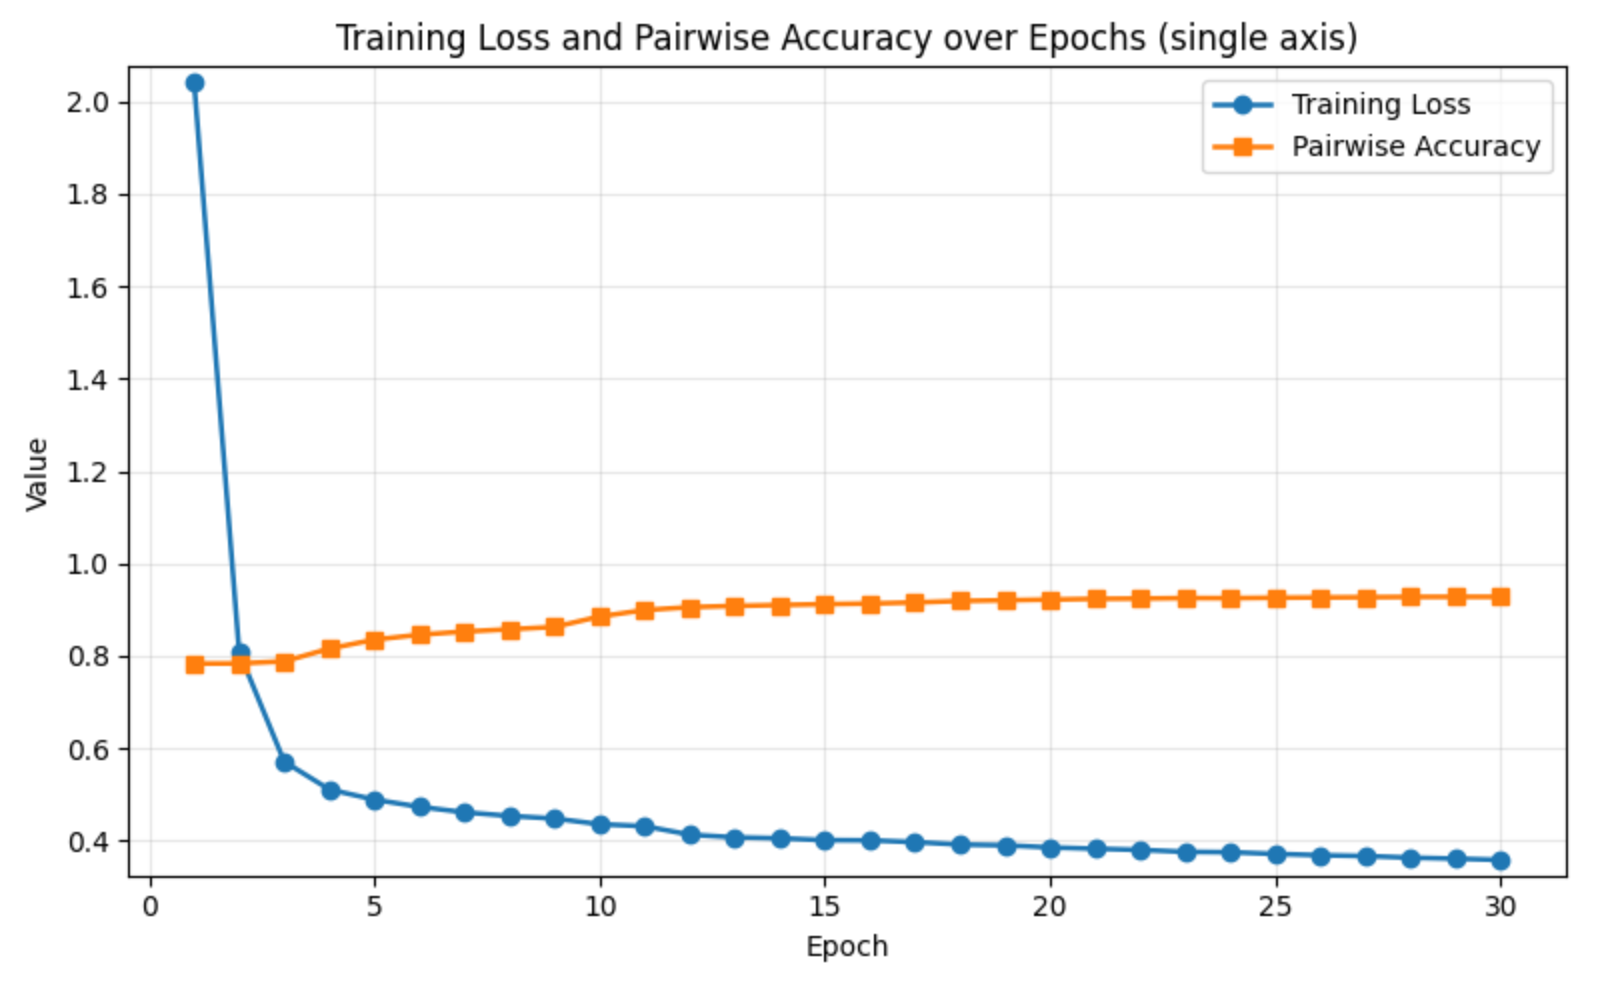
\includegraphics[width=0.5\linewidth]{image401.png}
    \caption{ConvNCF training loss and training accuracy over 30 epochs on Yelp dataset}
    \label{fig:convncf_yelp_train}
\end{figure}

\begin{figure}[H]
    \centering
    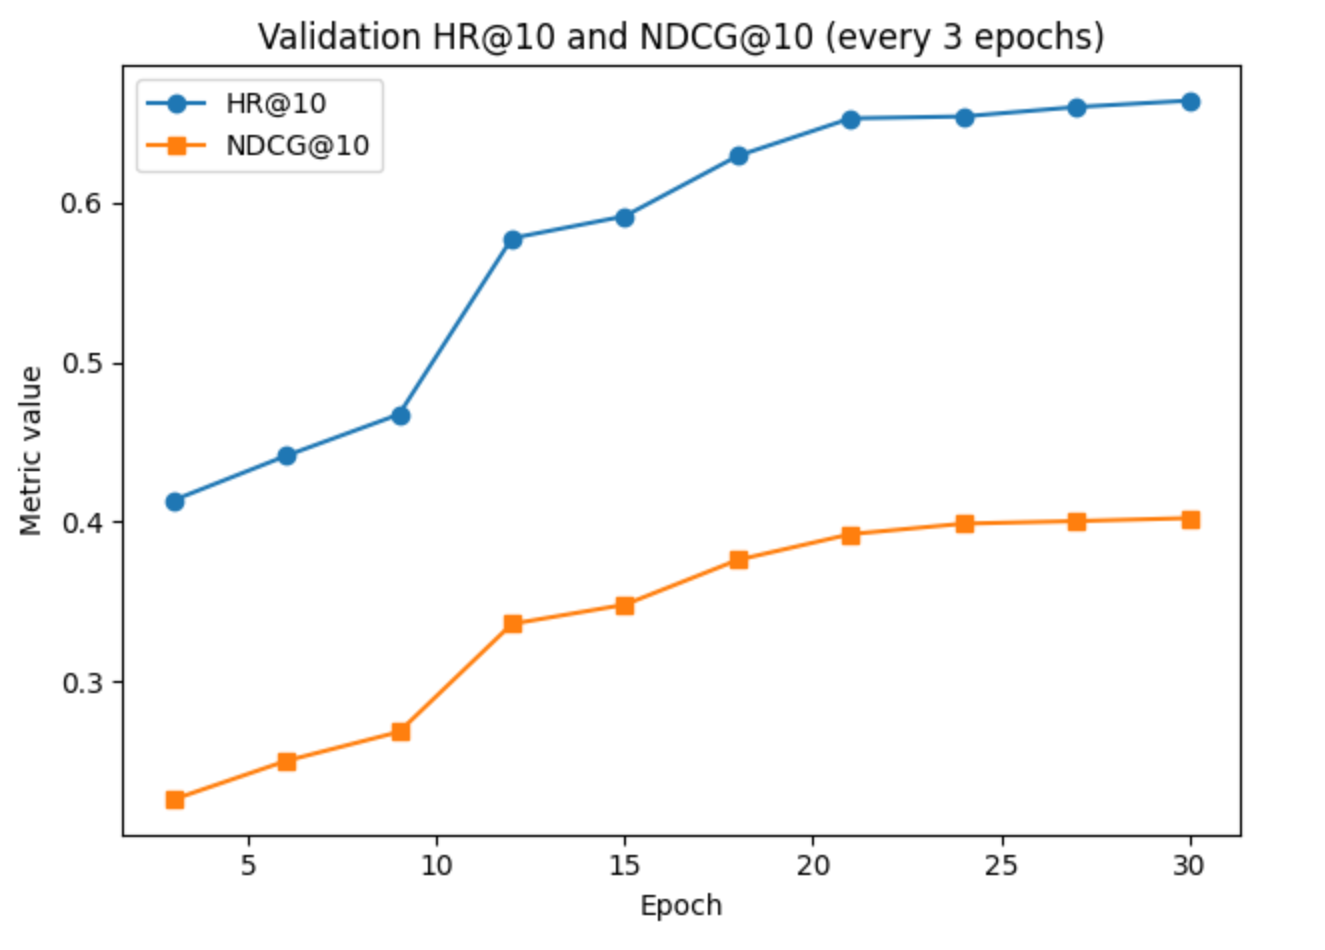
\includegraphics[width=0.5\linewidth]{image400.png}
    \caption{ConvNCF validation HR\@10 and NDCG\@10 over 30 epochs (every 3 epochs) on Yelp dataset}
    \label{fig:convncf_yelp_val}
\end{figure}


\subsection{NeuMF pretrained}

\subsubsection{MovieLens}
Table~\ref{tab:neumfpre_movielens_results} reports the test performance of the pretrained NeuMF model on the MovieLens. MLP and GMF were pretrained till convergence, then the weights were fit in the NeuMF model. Highest evaluated epoch is epoch 3. At this checkpoint, NeuMF-pre obtains \emph{HR@10} of $0.6480$ and \emph{NDCG@10} of $0.3814$, which is slightly higher than MLP and NeuMF without pretraining, but still marginally below GMF. As $K$ increases from $5$ to $20$, both metrics improve monotonically: \emph{HR@K} increases from $0.4778$ to $0.8137$, and \emph{NDCG@K} from $0.3248$ to $0.4201$.

\begin{table}[H]
\centering
\caption{NeuMF-pre Test Performance on the MovieLens Dataset at Best Epoch (Epoch 3)}
\label{tab:neumfpre_movielens_results}
\begin{tabular}{c c c}
\hline
\textbf{K} & \textbf{HR@K} & \textbf{NDCG@K} \\
\hline
5  & 0.4778 & 0.3248 \\
10 & 0.6480 & 0.3814 \\
20 & 0.8137 & 0.4201 \\
\hline
\end{tabular}
\end{table}
The training curves in Figure~\ref{fig:neumfpre_movielens_train} show that, starting from pretrained GMF and MLP weights, the NeuMF-pre model quickly achieves a low training loss and high training accuracy, after which both curves evolve only slowly. The validation metrics in Figure~\ref{fig:neumfpre_movielens_val} exhibit a familiar pattern: both \emph{HR@10} and \emph{NDCG@10} are highest at the beginning of fine-tuning and then decrease steadily over the remaining epochs. This again indicates overfitting during continued training, even with preinitialised weights.  The comparison with NeuMF without pretraining suggests that pretraining yields a consistent, but relatively modest, improvement on MovieLens.

\begin{figure}[H]
    \centering
    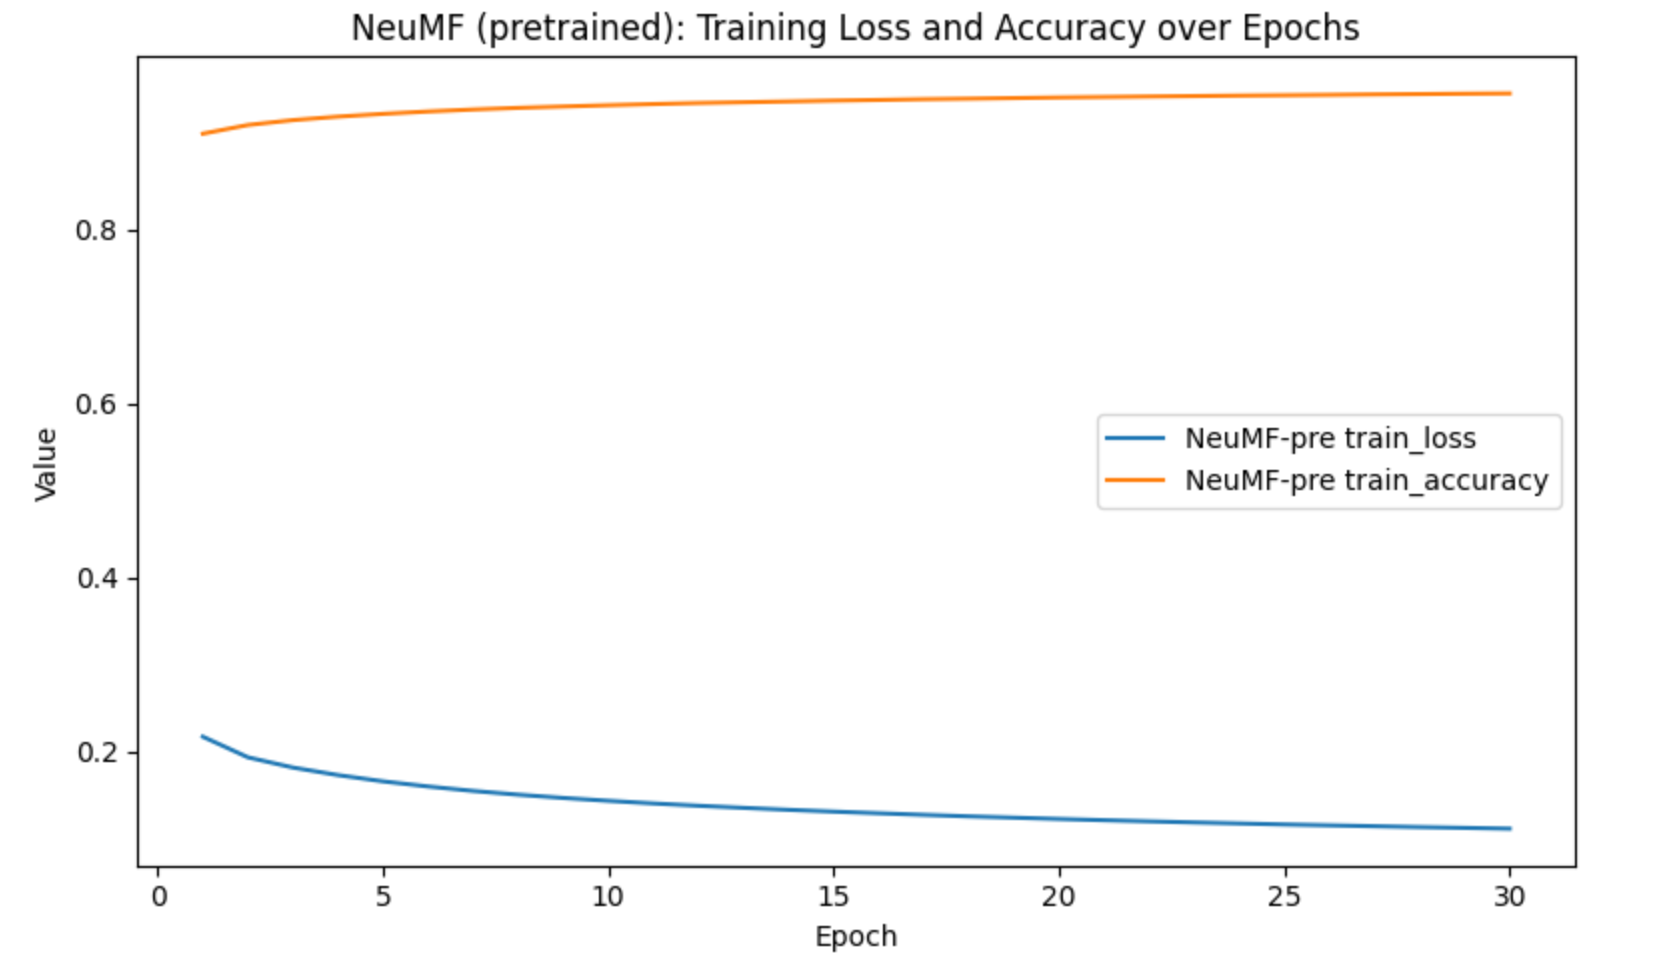
\includegraphics[width=0.5\linewidth]{image113.png}
    \caption{NeuMF-pre training loss and training accuracy over 30 epochs on MovieLens dataset}
    \label{fig:neumfpre_movielens_train}
\end{figure}
\begin{figure}[H]
    \centering
    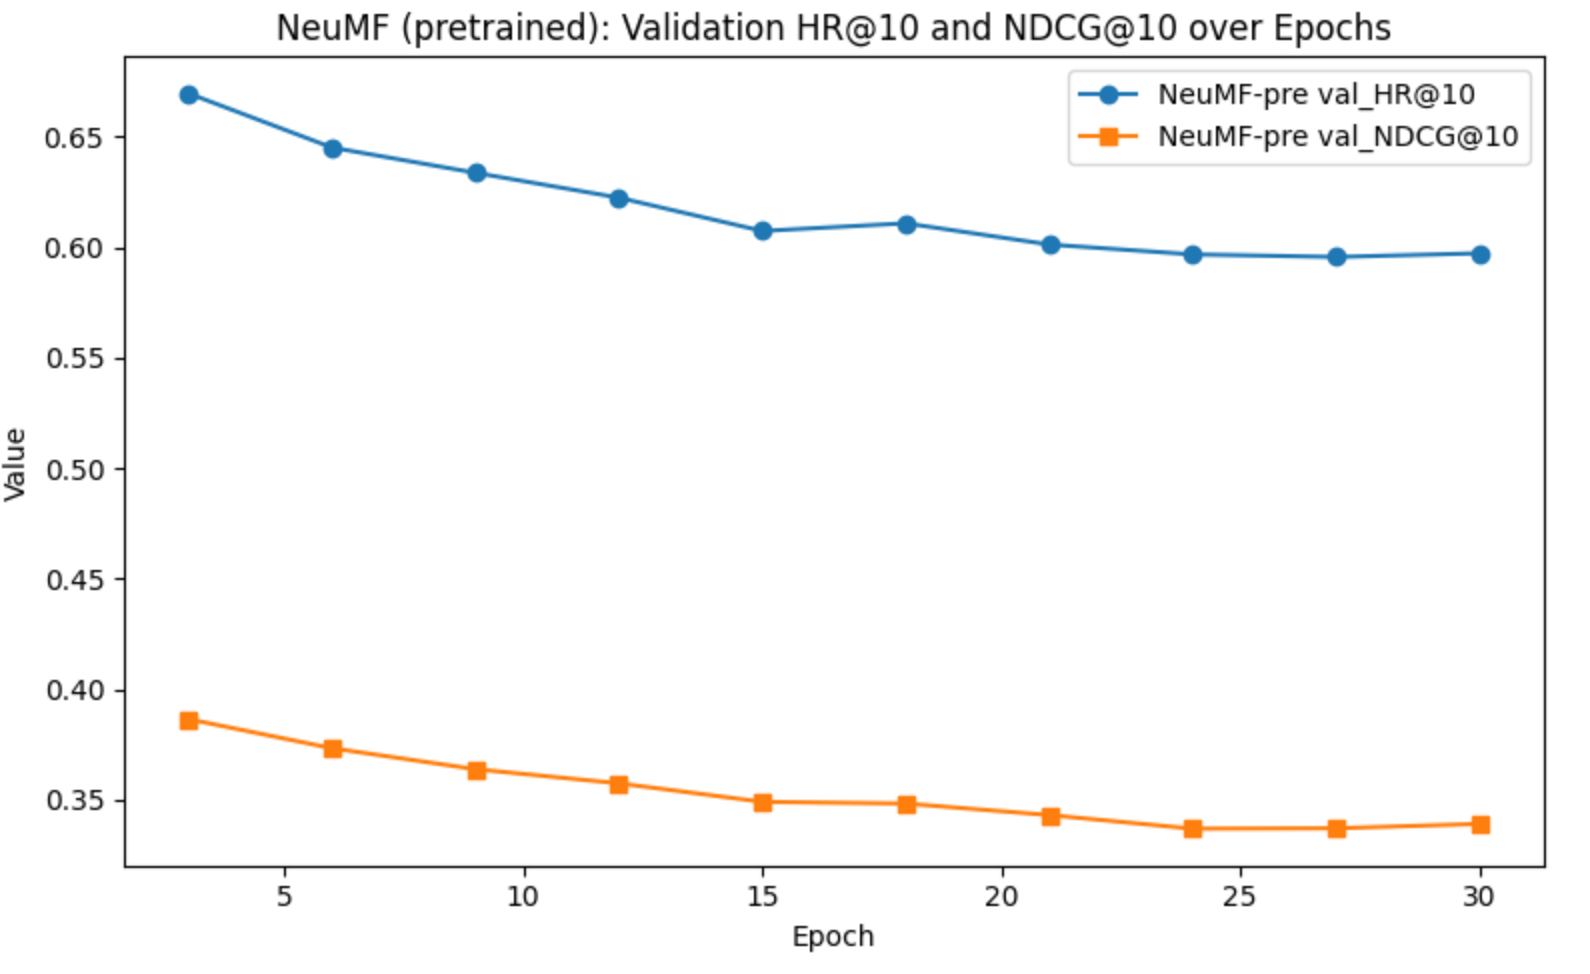
\includegraphics[width=0.5\linewidth]{image115.png}
    \caption{NeuMF-pre validation HR@10 and NDCG@10 over 30 epochs (every 3 epochs) on MovieLens dataset}
    \label{fig:neumfpre_movielens_val}
\end{figure}

\subsubsection{Yelp}
On the Yelp dataset, the pretrained NeuMF model is additionally tuned over the learning rate. A small grid is considered,
\[
\texttt{learning\_rate} \in \{10^{-4}, 5 \times 10^{-4}, 10^{-3}, 5 \times 10^{-3}\},
\]
and the configuration with the highest validation \emph{NDCG@10} is selected. The best performance is obtained with a learning rate of $10^{-4}$.

Table~\ref{tab:neumfpre_yelp_results} reports the test performance at the best validation epoch for this configuration (epoch 9). At $K=10$, NeuMF-pre achieves \emph{HR@10} of $0.6917$ and \emph{NDCG@10} of $0.4297$, improving slightly over NeuMF without pretraining and over the standalone GMF and MLP models. As before, performance increases with $K$, reaching \emph{HR@20} of $0.8236$ and \emph{NDCG@20} of $0.4659$.

\begin{table}[H]
\centering
\caption{NeuMF-pre Test Performance on the Yelp Dataset at Best Epoch (Epoch 9)}
\label{tab:neumfpre_yelp_results}
\begin{tabular}{c c c}
\hline
\textbf{K} & \textbf{HR@K} & \textbf{NDCG@K} \\
\hline
5  & 0.5391 & 0.3797 \\
10 & 0.6917 & 0.4297 \\
20 & 0.8236 & 0.4659 \\
\hline
\end{tabular}
\end{table}
The training curves in Figure~\ref{fig:neumfpre_yelp_train} show a healthy optimization process: the loss and accuracy converge to best values around epochs 15-20, after epoch 20 flattening out.

On the validation set (Figure~\ref{fig:neumfpre_yelp_train}), show that the optimal values of the metrics are around epochs 5-10: for the first few epochs we see an increase in the metrics, which is followed by a slow decrease, which suggest overfitting after epoch 10.

\begin{figure}[H]
    \centering
    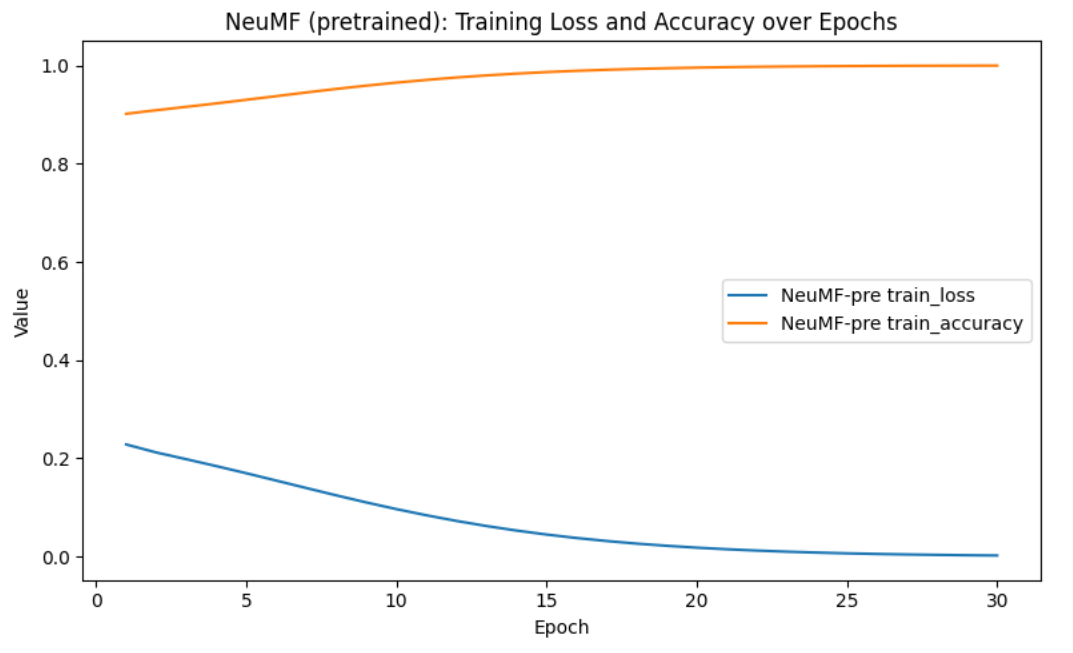
\includegraphics[width=0.5\linewidth]{image119.png}
    \caption{NeuMF-pre training loss and training accuracy over 30 epochs on Yelp dataset}
    \label{fig:neumfpre_yelp_train}
\end{figure}
\begin{figure}[H]
    \centering
    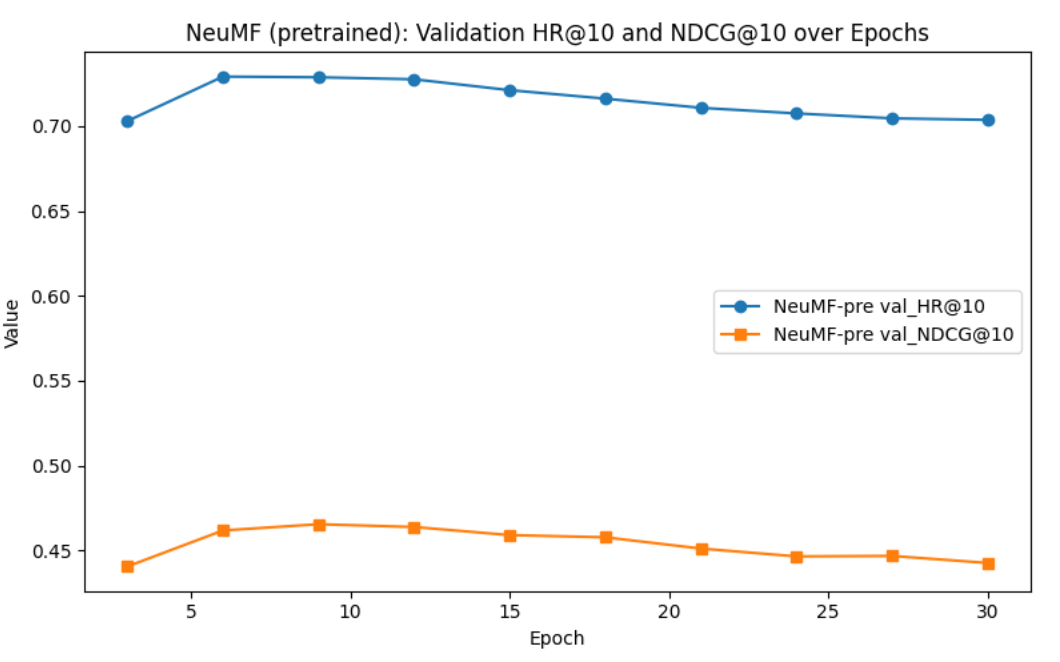
\includegraphics[width=0.5\linewidth]{image120.png}
    \caption{NeuMF-pre validation HR@10 and NDCG@10 over 30 epochs (every 3 epochs) on Yelp dataset}
    \label{fig:neumfpre_yelp_val}
\end{figure}



\section{Combined results}
All results were summarized in two table (one for each datasets) to address main results.
\begin{table}[H]
\centering
\caption{Summary of test HR@K and NDCG@K for all models on the MovieLens dataset in decreasing order}
\label{tab:summary_movielens}
\begin{tabular}{lcccccc}
\hline
\textbf{Model} & \textbf{HR@5} & \textbf{NDCG@5} & \textbf{HR@10} & \textbf{NDCG@10} & \textbf{HR@20} & \textbf{NDCG@20} \\
\hline
GMF        & 0.4758 & 0.3239 & \textbf{0.6629} & \textbf{0.3853} & \textbf{0.8192} & \textbf{0.4279} \\
NeuMF-pre  & \textbf{0.4778} & \textbf{0.3248} & 0.6480 & 0.3814 & 0.8137 & 0.4201 \\
NeuMF      & 0.4684 & 0.3170 & 0.6457 & 0.3752 & 0.8103 & 0.4158 \\
MLP        & 0.4568 & 0.3078 & 0.6358 & 0.3675 & 0.8053 & 0.4115 \\


KNN        & 0.3652 & 0.2521 & 0.5204 & 0.3022 & 0.7017 & 0.3482 \\
MF-BPR     & 0.3634 & 0.2409 & 0.5379 & 0.2989 & 0.7300 & 0.3460 \\
ConvNCF    & 0.1838 & 0.1163 & 0.3220 & 0.1606 & 0.5040 & 0.2071 \\
\hline
\end{tabular}
\end{table}


\begin{table}[H]
\centering
\caption{Summary of test HR@K and NDCG@K for all models on the Yelp dataset in decreasing order}
\label{tab:summary_yelp}
\begin{tabular}{lcccccc}
\hline
\textbf{Model} & \textbf{HR@5} & \textbf{NDCG@5} & \textbf{HR@10} & \textbf{NDCG@10} & \textbf{HR@20} & \textbf{NDCG@20} \\
\hline
KNN        & \textbf{0.5933} & \textbf{0.4320} & \textbf{0.7301} & \textbf{0.4747} & \textbf{0.8461} & \textbf{0.5050} \\
NeuMF-pre  & 0.5391 & 0.3797 & 0.6917 & 0.4297 & 0.8236 & 0.4659 \\
GMF        & 0.5345 & 0.3800 & 0.6775 & 0.4284 & 0.8039 & 0.4578 \\
NeuMF      & 0.5371 & 0.3794 & 0.6744 & 0.4264 & 0.7919 & 0.4555 \\
MLP        & 0.5195 & 0.3688 & 0.6787 & 0.4224 & 0.8162 & 0.4558 \\
ConvNCF    & 0.4624 & 0.3172 & 0.6242 & 0.3702 & 0.7825 & 0.4121 \\
MF-BPR     & 0.3235 & 0.2296 & 0.4329 & 0.2666 & 0.5572 & 0.2958 \\

\hline
\end{tabular}
\end{table}


\textbf{MLP-based models.} A main takeaway from these tables is that MLP-based models, such as NeuMF and the standalone MLP, are not necessarily better than MF models. As can be seen in Tables~\ref{tab:summary_movielens} and~\ref{tab:summary_yelp}, they are consistently outperformed by the simpler GMF variant in terms of \emph{NDCG@K}. This indicates that, without careful hyperparameter tuning of deep models (which is extremely computationally expensive), MLP-based architectures do not automatically translate their higher capacity into better ranking quality. Instead, the learning curves suggest that they tend to memorise noise: training pairwise accuracy quickly approaches $1.0$ while validation \emph{HR@10} and \emph{NDCG@10} peak in the first few epochs and then decline, indicating overfitting rather than successful exploitation of non-linear relationships in the data.

This observation is consistent with the argument of Rendle et al.~\cite{rendle2020neural} that well-tuned MF models often outperform deep neural recommenders on sparse implicit-feedback datasets such as MovieLens or Yelp. Anelli et al.~\cite{anelli2021reenvisioning} further show that, when the original NeuMF comparisons are carefully replicated and extended, MF-style methods remain highly competitive in terms of accuracy, while neural models mainly distinguish themselves on beyond-accuracy dimensions such as coverage, diversity, and novelty. In other words, whether a neural architecture is preferable to MF depends strongly on which aspects of recommendation quality are emphasised.

On MovieLens, GMF achieves the highest \emph{NDCG@K} across all cut-offs, with \emph{NDCG@10} of $0.3853$ and \emph{NDCG@20} of $0.4279$, while NeuMF-pre and NeuMF trail slightly behind (Table~\ref{tab:summary_movielens}). The standalone MLP model performs worse still, despite having more parameters than GMF and being trained under the same optimisation setup. On Yelp, the picture is similar, although the gaps are smaller. NeuMF-pre attains the best scores among the neural models (\emph{NDCG@10} $= 0.4297$, \emph{NDCG@20} $= 0.4659$), with NeuMF, GMF, and MLP forming a tight cluster just below it (Table~\ref{tab:summary_yelp}). The improvements from pretraining are thus present but modest, and none of the MLP-based variants dominates the MF-style GMF across all accuracy metrics. Given that the validation plots reveal strong overfitting for GMF, MLP, and NeuMF on Yelp as well, these results support the view that model capacity is not the main bottleneck on such sparse implicit-feedback data.

Overall, the empirical evidence from both datasets reinforces the conclusion that MLP-based recommenders require substantial tuning effort (learning rates, regularization, architecture depth, negative sampling, etc.) to outperform well-regularized MF baselines. Within the experimental regime considered in this thesis (fixed embedding size, limited grid search, and early stopping based on \emph{NDCG@10}), the benefits of adding deep non-linear layers are relatively small and sometimes even negative, which aligns with prior critical evaluations of neural recommenders in the literature~\cite{rendle2020neural,anelli2021reenvisioning}. It also reflects that the evaluation in this thesis focuses purely on accuracy-oriented metrics; potential advantages of neural models in terms of coverage or diversity, highlighted by Anelli et al.~\cite{anelli2021reenvisioning}, are outside the present scope.





\textbf{Is ConvNCF a good fit?}
    we can clearly state that the ConvNCF model performs better for Yelp dataset, as well as the KNN model, this can be a results of a Yelp dataset being more spatial related, since there is a geographical relationship in the data. which, indeed makes ConvNCF perform better, by making more clear patterns in the data. By comparing the \ref{fig:norm_heat_Yelp} and \ref{fig:norm_heat_Movie} we can see that there are better visual patterns formed in the Yelp dataset, than in the MovieLens dataset.
\begin{figure}[H]
    \centering
    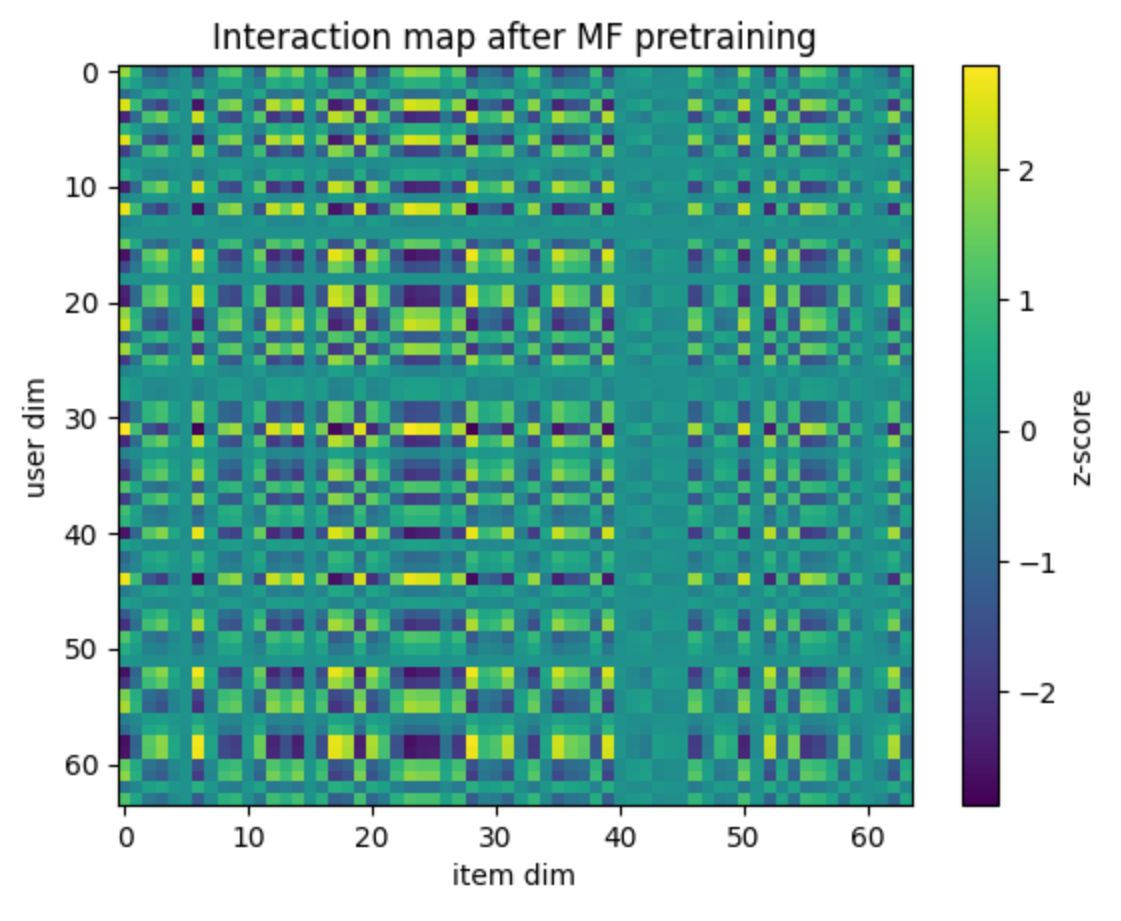
\includegraphics[width=0.5\linewidth]{image10000.png}
    \caption{Heat map of embedded user and item vectors after pretraining the MF model for 15 epochs on Yelp dataset.}
    \label{fig:norm_heat_Yelp}
\end{figure}
%%% Add the MovieLens map to
\begin{figure}[H]
    \centering
    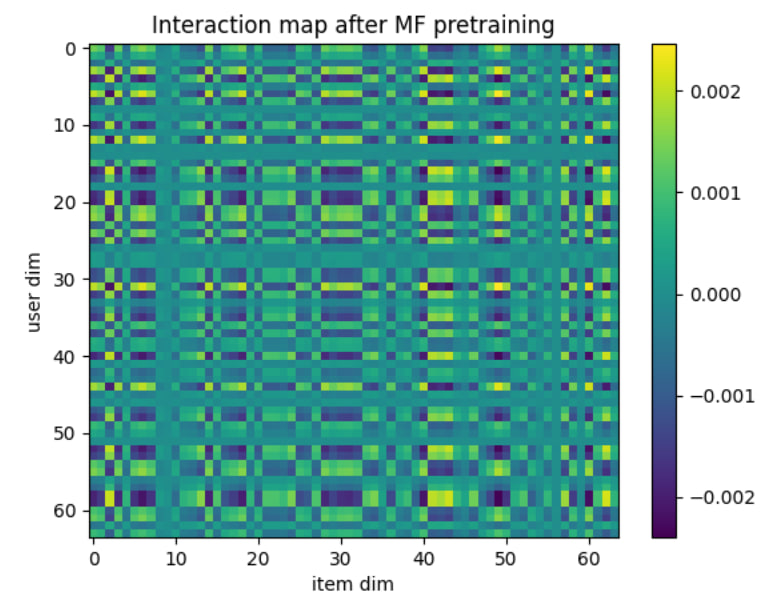
\includegraphics[width=0.5\linewidth]{image999.png}
    \caption{Heat map of embedded user and item vectors after pretraining the MF model for 15 epochs on MovieLens dataset.}
    \label{fig:norm_heat_Movie}
\end{figure}
However, a conceptually simple and finely-tuned baseline model, such as Item-based K-Nearest Neighbors (KNN), was observed to significantly outperform the ConvNCF model, even on a dataset hypothesized to be favorable to CNN architectures. This performance disparity raises a critical question regarding the necessity and complexity of the ConvNCF approach, which requires substantially more computational resources and extensive hyperparameter tuning yet yields inferior results.

On the other hand, The ConvNCF model shows weak results on the MovieLens dataset, which lacks the any structural patterns (semantic-geographical connections) found in Yelp.

This poor performance reinforces the critique that the CNN architecture is an unsuitable choice for general recommendation data. Since, the outer product barely has any spatial features the CNN cannot effectively extract the spatial features it was designed for, leading to a performance drop.

This finding aligns with a major architectural critique articulated by Anelli et al. (and Ferrari Dacrema et al. in related work)~\cite{anelli2020reenvisioning}. These works argue that the fundamental assumption required for CNNs to be effective—the presence of meaningful spatial locality—is not met by the outer-product interaction map. Unlike images, where shifting a row or column structurally damages the visual information, the indices of the latent dimensions in the user and item embeddings are arbitrary and interchangeable. Consequently, the convolution filters cannot reliably extract spatially invariant features. The ability of ConvNCF to produce any effective result is therefore attributed not to its spatial feature extraction capabilities, but rather to the CNN merely acting as a highly complex, non-linear feature transformation function that increases model complexity without a commensurate gain in predictive power.

\textbf{Is deep learning helpful?}
From these tables we can draw a nuanced answer. On MovieLens, moving from classical non–neural baselines (KNN, MF-BPR) to latent-factor neural models clearly helps: GMF, NeuMF and MLP all improve both \emph{HR@10} and \emph{NDCG@10} by a seizable margin. For instance, GMF reaches \emph{HR@10} $=0.6629$ and \emph{NDCG@10} $=0.3853$, compared with $0.5204/0.3022$ for KNN and $0.5379/0.2989$ for MF-BPR, i.e., roughly a 25–30\% relative gain in ranking quality. This suggests that learning low-dimensional user and item embeddings with a trainable interaction function is indeed beneficial on this denser dataset.

However, within the family of neural models, increased depth does not systematically translate into better performance. The shallow GMF model, which can be seen as a lightly generalized MF, attains the best \emph{NDCG@K} across all cut-offs on MovieLens, while NeuMF-pre, NeuMF and the standalone MLP only match or slightly trail it. On Yelp, all four neural MF-style models (GMF, MLP, NeuMF, NeuMF-pre) form a tight cluster, but none of them is able to outperform the strong KNN baseline, which remains best in every column of Table~\ref{tab:summary_yelp}. The convolution ConvNCF architecture performs particularly poorly on MovieLens and only reaches mid-range performance on Yelp, despite being the most complex model in the comparison.

Taken together, these results indicate that deep learning is helpful in the limited sense that embedding-based MF models (GMF) can significantly outperform simple memory-based or point-wise MF baselines, especially on MovieLens. At the same time, additional architectural sophistication (deeper MLP branches, convolution over outer products) does not automatically yield further gains and can even hurt performance when hyperparameters are not extensively tuned. This aligns with prior work such as Rendle et al.~\cite{rendle2020neural} and Anelli et al.~\cite{anelli2021reenvisioning}, which argue that well-regularized MF-style models often remain competitive with, or superior to, more complex neural recommenders once evaluation and tuning are controlled for. 

Thus, we can conclude that NeuMF-pre has potential to be the benchmark model across both datasets, but ConvNCF cannot be, since it only works (to some extent) on Yelp dataset.




























  
\section{Conclusions and discussions}

\subsection{Limitations}

The conclusions of this study must be interpreted in light of several important limitations of the experimental design.

\textbf{Restricted hyperparameter optimization.}  
    Deep models are notoriously sensitive to hyperparameters (learning rate, regularization strength, models' depth, negative sampling strategy, optimizer choice, etc.). In this thesis, hyperparameter optimization was intentionally restricted to keep the comparison computationally feasible. A single embedding size ($k=64$), a fixed batch size, a single negative sampling rate for most models, and relatively small grids over learning rates and $\ell_2$ penalties were used. Architectural choices such as the number of hidden layers and layer width in the MLP branch were kept fixed rather than tuned per dataset. It is therefore plausible that more aggressive hyperparameter search could further improve the performance of NeuMF and MLP, and potentially change some rankings between neural models.

\textbf{Training horizon and convergence.}  
    For most models, the maximum number of epochs was capped at $30$ (and at $50$ for MF-BPR) due to time constraints, whereas the original ConvNCF paper reports training deep CNN variants for up to $1\,500$ epochs and original NeuMF reports 50 epochs. Several learning curves, particularly for MF-BPR and ConvNCF on Yelp, suggest that the models were still improving at the end of training and had not fully converged. Conversely, for GMF, MLP, NeuMF, and NeuMF-pre, the validation curves peak very early and then deteriorate, indicating strong overfitting. This means that simply increasing the epoch budget without substantial changes in regularization and optimization would not necessarily improve generalization, but it does highlight that the models were not explored in their full capacity, suggested in the original papers.

\textbf{ConvNCF architecture choice.}  
    The ConvNCF experiments used a shallow CNN variant rather than the deepest configuration from the original paper. In preliminary experiments, deeper ConvNCF models with more convolution layers were found to be even more unstable on both MovieLens and Yelp: they either failed to decrease the loss or collapsed in training accuracy, even after tuning $\ell_2$ regularization. As a result, the final experiments focus on a shallow ConvNCF configuration that exhibited at least some signs of learning. The conclusions of the thesis therefore apply to feasible shallow ConvNCF under limited tuning, not to a full reproduction of the original deep architecture under very long training times.

 \textbf{Negative sampling design.}  
    The negative sampling strategy was deliberately kept simple and uniform across models: for most architectures, four negative items were sampled per positive interaction (\texttt{num\_neg} = 4), whereas MF-BPR was originally proposed with a single negative per positive in~\cite{rendle2012bpr}. Using a higher negative sampling rate may have affected MF-BPR performance, particularly on the sparser Yelp dataset, where the ratio of observed to unobserved interactions is extremely low. For ConvNCF on Yelp, the negative sampling rate was reduced to \texttt{num\_neg} = 1 to control training time. Exploring \texttt{num\_neg} tuning for the MF-BPR and ConvNCF or using  more sophisticated sampling strategies (for example popularity-based or adaptive hard negative sampling) could yield different conclusions about the relative strengths of pairwise vs point-wise optimized models.



\subsection{Future work}

Future work could extend this study along several directions. First, a more systematic hyperparameter search and longer training schedules would provide a clearer picture of the best achievable performance of each architecture under a fixed computational budget. Second, incorporating additional models such as LightGCN, NGCF, and state-of-the-art sequential recommenders would allow a more comprehensive comparison between graph-based, sequential, and neural MF-style approaches. Finally, extending the analysis to  cold-start conditions would further test the generality of the conclusions drawn here.
\subsection{Conclusion}

This thesis set out to investigate whether deep neural collaborative filtering models such as NeuMF and ConvNCF provide a substantial accuracy advantage over simpler matrix factorization baselines when evaluated under a controlled experimental setup on two widely used implicit-feedback datasets, MovieLens-1M and Yelp. All models were trained and evaluated under a common leave-one-out protocol with top-$K$ ranking metrics (\emph{HR@K}, \emph{NDCG@K}), and particular care was taken to include strong classical baselines such as item-based KNN and MF-BPR.

Across both datasets, the empirical results paint a consistent picture. On MovieLens, the shallow neural MF variant (GMF) performs best among all models in terms of \emph{NDCG@K}, with NeuMF-pre and NeuMF following closely behind and the standalone MLP slightly worse. On Yelp, where the data are much sparser and has some geographical related semantics the conceptually simple ItemKNN baseline achieves the highest \emph{HR@K} and \emph{NDCG@K}, while GMF, MLP, NeuMF, and NeuMF-pre form a tight cluster just below it. The ConvNCF model performs particularly poorly on MovieLens and only reaches mid-range performance on Yelp, despite being the most complex architecture in the comparison. These findings support the conclusion that, under realistic tuning and compute constraints, deep neural recommenders do not automatically dominate well-regularized MF-based models and neighborhood baselines.

More specifically, the results show that some extent of deep learning helps, like in the GMF but more depth or architectural complexity does not necessarily translate into better ranking quality.



\addcontentsline{toc}{section}{References}
\bibliographystyle{plain}
\bibliography{references}


\end{document}
